% manuscript_main.tex
% P1 — Meteorology value for PM10 multi-horizon forecasting
% Target journal: Atmospheric Research (Elsevier, ISSN 0169-8095)
% Compile: pdflatex → bibtex → pdflatex × 2
%
% Figures are referenced from ../results/
% Build from repo root: pdflatex manuscripts/manuscript_main.tex

\documentclass[12pt,a4paper]{article}

\usepackage[utf8]{inputenc}
\usepackage[T1]{fontenc}
\usepackage{lmodern}
\usepackage[margin=2.5cm]{geometry}
\usepackage{setspace}
\doublespacing
\usepackage{lineno}
\linenumbers
\usepackage{graphicx}
\usepackage{booktabs}
\usepackage{amsmath}
\usepackage{amssymb}
\usepackage{natbib}
\bibliographystyle{abbrvnat}
\usepackage{hyperref}
\hypersetup{colorlinks=true, linkcolor=blue, citecolor=blue, urlcolor=blue}
\usepackage{caption}
\usepackage{subcaption}
\usepackage{array}
\usepackage{rotating}
\usepackage{siunitx}
\usepackage{xcolor}

% ── title block ───────────────────────────────────────────────────────────────

\title{Does meteorology extend the useful forecast horizon for urban
\PMten{}?\
A multi-city, multi-horizon skill analysis with XGBoost and SARIMA}

\newcommand{\PMten}{PM\textsubscript{10}}

\author{
  Federico García Crespí\textsuperscript{1}\thanks{Corresponding author.
    \texttt{fedeg@umh.es}} \\[6pt]
  \textsuperscript{1}Universidad Miguel Hernández de Elche, Spain
}

\date{}

% ── document ──────────────────────────────────────────────────────────────────

\begin{document}

\maketitle

\begin{abstract}
\noindent
Accurate multi-horizon forecasting of \PMten{} concentrations is increasingly
important as regulators tighten ambient air quality standards.  This study
asks whether retrospective meteorological information extends the useful
forecast horizon $H^*$ when comparing a lags-only information set against a
lags+meteorology information set constructed from concurrent
observations.  We apply a rolling-origin expanding-window backtesting protocol
(January 2020 -- July 2023) at two European settings: Madrid Casa de Campo
(Spain) and a network of eight monitoring stations in Ireland.  Three model
classes are evaluated at each of $h = 1, \ldots, 24$ lead hours: (i) a
persistence baseline, (ii) SARIMA(1,0,1)(1,0,0)$_{24}$ as a linear statistical
reference, and (iii) XGBoost fitted separately for each horizon, once with
\PMten{} lags only (\textit{lags only}) and once with lags plus nine
meteorological covariates treated as retrospectively observed at the forecast
origin (\textit{lags + met.}).  Forecast quality is measured via the RMSE skill
score relative to persistence; $H^*$ is determined under the primary strict
criterion $H^*_{\text{strict,max-run}}$ (longest contiguous positive-skill run
located anywhere within $h = 1, \ldots, 24$), with auxiliary variants reported
separately.

At Madrid, the XGBoost $H^*_{\text{strict,max-run}}$ changes from 10~h
($h=15$--24) under lags-only to 21~h ($h=4$--24) under lags+meteorology, an
observed maximum-run-length difference of $\Delta H^*=+11$~h (not an endpoint
extension).  A paired timestamp-safe moving-block bootstrap shows substantial
sampling variability (median $+2$~h; 95\% percentile interval $[0,+14]$~h;
$P(\Delta H^*>0)=0.758$).  In Ireland, seven of eight stations reach the 24-h
ceiling under lags-only, and the network mean changes only from 23.8~h to
23.9~h (mean $\Delta H^*=+0.1$~h).  Across 36 planned site--horizon comparisons, 33 DM tests were valid.
After global Benjamini--Hochberg correction over the 33 valid tests, only
Birr at $h=1$ remained significant
(DM $=3.71$, $p_{\mathrm{raw}}=0.00027$,
$q_{\mathrm{BH}}=0.0088$).
Horizon-specific inferential evidence was therefore sparse and localized.
These results indicate that the incremental value of
retrospective meteorological information is strongly horizon- and
site-dependent.  Because the meteorological inputs are retrospective
observations rather than origin-time weather forecasts, the findings should be
interpreted as an upper bound on potential information value rather than as
demonstrated operational skill.

\medskip
\noindent
\textbf{Keywords:} PM\textsubscript{10}; atmospheric aerosol; boundary layer;
meteorological covariates; forecast horizon; XGBoost; SARIMA; skill score;
Diebold--Mariano test; air quality.
\end{abstract}

\newpage

% ─────────────────────────────────────────────────────────────────────────────
\section{Introduction}
\label{sec:intro}
% ─────────────────────────────────────────────────────────────────────────────

Particulate matter with aerodynamic diameter below 10~\si{\micro\metre}
(\PMten{}) is the dominant coarse aerosol fraction in the urban boundary layer
and one of the most consequential atmospheric pollutants in European cities.
Its surface concentration integrates contributions from primary crustal and
traffic-related emissions, long-range transported dust, and secondary aerosol
formation, all modulated by boundary-layer mixing, wet scavenging, and
synoptic-scale advection \citep{Seinfeld2006, Kumar2016}.  Sustained exposure
is associated with cardiovascular and respiratory morbidity, premature
mortality, and reduced quality of life \citep{WHO2021, EEA2023}.  The European
regulatory framework has progressively tightened in response: Directive
2008/50/EC established the current limit of
40~\si{\micro\gram\per\cubic\metre} as an annual mean, and the revised
Directive 2024/2881/EU, which entered into force in December 2024, halves that
threshold to 20~\si{\micro\gram\per\cubic\metre} by 2030 \citep{EU2024_2881}.
Against this backdrop, accurate \PMten{} forecasts are increasingly valuable
both for triggering episode-specific abatement measures and for guiding
longer-term urban planning.

The temporal evolution of near-surface \PMten{} is tightly coupled to
boundary-layer dynamics.  Under stable nocturnal or anticyclonic conditions,
the mixing layer is shallow and aerosol concentrations build up through
in-situ accumulation, producing high lag-1 autocorrelation.  Conversely,
deep daytime convective mixing, frontal passages, and precipitation scavenging
all accelerate aerosol dispersal, reducing persistence.  Wind speed and
direction govern horizontal transport of aerosol plumes from upwind sources,
while relative humidity influences hygroscopic growth and optical properties
of the coarse fraction \citep{Seinfeld2006, Kumar2016}.  This physical coupling
motivates the hypothesis that incorporating meteorological predictors into
statistical or machine-learning forecasting models should improve forecast
skill, particularly at medium-to-long lead times where the aerosol signal can
no longer be extrapolated from its recent history alone.

Empirical evidence, however, is mixed.  Several studies report clear gains
when meteorological inputs are added to machine-learning forecasting models:
\citet{Pak2018} found substantial improvements from boundary-layer variables
for PM prediction in Korea, and \citet{Bai2018} demonstrated that wavelet
decomposition of meteorological inputs improved short-range pollutant
forecasts in China.  Other studies find that lagged pollutant concentrations
already capture most of the predictable variance, leaving little room for
meteorology to contribute at sub-daily lead times.  This inconsistency across
the literature likely reflects differences in local autocorrelation structure,
data availability, and the choice of forecast horizon — factors that are
rarely disentangled in a single study.

The \emph{forecast horizon problem} is central to practical decision-making in
air quality management.  Operators of early-warning systems need to know not
only whether a model is skilful on average, but over which range of lead times
it reliably outperforms a naïve benchmark.  We operationalize useful
forecastability through $H^*_{\mathrm{strict,max-run}}$, defined as the length
of the longest contiguous sequence of lead times with positive skill relative to
persistence within the evaluated $h=1,\ldots,24$ window.  The central question
of this paper is whether, and by how much, adding retrospective meteorological
information changes the longest contiguous positive-skill run for \PMten{}, and
whether observed site-level differences are associated with local persistence
characteristics.

To answer this question we conduct a controlled multi-city comparison.
Madrid Casa de Campo (Spain) and a network of eight stations in Ireland provide
contrasting urban environments with different meteorological regimes and
\PMten{} autocorrelation structures.  We evaluate three model classes —
persistence, SARIMA, and XGBoost — under a strict leakage-free
rolling-origin protocol and use the Diebold--Mariano test
\citep{Diebold1995} to assess whether observed skill differences
are statistically distinguishable.

The remainder of this paper is structured as follows.  Section~\ref{sec:data}
describes the datasets and preprocessing.  Section~\ref{sec:methods} presents
the backtesting protocol, model specifications, and evaluation metrics.
Section~\ref{sec:results} reports skill curves, $H^*$ estimates, and
significance tests for both sites.  Section~\ref{sec:discussion} interprets
the results in terms of the autocorrelation-persistence mechanism.
Section~\ref{sec:conclusions} summarises the main findings and their
operational implications.

% ─────────────────────────────────────────────────────────────────────────────
\section{Data}
\label{sec:data}
% ─────────────────────────────────────────────────────────────────────────────

\subsection{Madrid}

Hourly \PMten{} concentrations and concurrent meteorological measurements were
obtained for Madrid Casa de Campo from the Madrid City Council open-data portal.
The station is classified as an urban-background site on the western edge of
the city, away from major point sources, and is representative of citywide
background conditions.  The study period spans January 2020 through July 2023;
records with missing \PMten{} or meteorological data were flagged and excluded
from model training and evaluation on a per-origin basis.  Nine meteorological
variables were retained: precipitation (\textit{rain}), temperature
(\textit{temp}), wet-bulb temperature (\textit{wetb}), dew-point temperature
(\textit{dewpt}), vapour pressure (\textit{vappr}), relative humidity
(\textit{rhum}), mean sea-level pressure (\textit{msl}), wind speed
(\textit{wdsp}), and wind direction (\textit{wddir}).

The lag-1 autocorrelation of hourly \PMten{} at Madrid over the training
period (2020--2022) is $\rho_1 = 0.957$, indicative of a highly persistent
series dominated by slow, boundary-layer-driven accumulation and dispersal
episodes lasting tens of hours.

\subsection{Ireland}

Hourly \PMten{} concentrations and meteorological covariates were obtained from
the Irish Environmental Protection Agency (EPA) monitoring network.  Eight
stations distributed across Ireland were selected on the basis of data
completeness over the study window (January 2020 -- July 2023):
Birr (Co.\ Offaly), Dublin Airport, Dundalk (Co.\ Louth), Pearse Street
Dublin, Ringsend Dublin, Edenderry (Co.\ Offaly), Henry Street Limerick, and
Portlaoise (Co.\ Laois).  The same nine meteorological variables used for
Madrid were extracted from the nearest EPA synoptic station for each monitoring
site.

Table~\ref{tab:descriptive} summarises the basic \PMten{} statistics for all
nine sites over the training and evaluation periods.  Concentrations are
generally low to moderate, with training-period means ranging from
11.3~\si{\micro\gram\per\cubic\metre} (Portlaoise) to
19.1~\si{\micro\gram\per\cubic\metre} (Dublin Airport), and Madrid at
18.4~\si{\micro\gram\per\cubic\metre}.  The 95th percentile values indicate
that episode concentrations above 40~\si{\micro\gram\per\cubic\metre} occur
at most stations, underscoring the operational relevance of medium-horizon
forecasting.  Data completeness is high: missing rates are below 2\% at all
sites during both periods.

\begin{table}[htbp]
\centering
\caption{Descriptive statistics of hourly \PMten{}
  (\si{\micro\gram\per\cubic\metre}) for all nine sites.
  Training: 2020--2022; evaluation: Jan--Jul 2023.
  $n$: valid hourly observations; miss: missing rate (\%).}
\label{tab:descriptive}
\small
\begin{tabular}{lrrrrrrrr}
\toprule
 & \multicolumn{4}{c}{Training (2020--2022)} & \multicolumn{4}{c}{Evaluation (2023)} \\
\cmidrule(lr){2-5}\cmidrule(lr){6-9}
Station & $n$ & Mean & SD & P95 & $n$ & Mean & SD & P95 \\
\midrule
Madrid              & 25\,630 & 18.4 & 20.0 & 42.0 & 4\,988 & 15.9 & 12.3 & 34.6 \\
\midrule
Birr                & 20\,372 & 12.8 & 12.5 & 31.4 & 5\,085 & 13.2 & 11.3 & 31.2 \\
Dublin Airport      & 21\,958 & 19.1 & 16.1 & 46.9 & 3\,504 & 15.7 & 10.9 & 34.3 \\
Dundalk             & 21\,938 & 11.4 &  8.6 & 24.3 & 3\,658 & 13.1 & 10.2 & 30.7 \\
Pearse St.\ Dublin  & 17\,009 & 13.0 &  9.9 & 30.2 & 5\,088 & 15.4 & 10.1 & 33.3 \\
Ringsend Dublin     & 21\,949 & 15.6 & 16.1 & 41.9 & 5\,087 & 14.0 & 13.1 & 36.7 \\
Edenderry           & 11\,526 & 17.8 & 19.8 & 48.8 & 5\,029 & 15.9 & 16.0 & 38.5 \\
Henry St.\ Limerick & 13\,128 & 13.0 & 12.1 & 30.8 & 5\,052 & 11.9 &  8.6 & 27.2 \\
Portlaoise          & 21\,958 & 11.3 &  9.7 & 27.5 & 5\,088 & 10.9 &  7.9 & 25.1 \\
\bottomrule
\end{tabular}
\end{table}

Across the eight Irish stations, the mean lag-1 autocorrelation of hourly
\PMten{} over the training period (2020--2022) is $\bar{\rho}_1 = 0.850$
(range: 0.804--0.945), reflecting a more moderately persistent pollution
regime compared with Madrid ($\rho_1 = 0.957$).  Dundalk (Co.\ Louth) is an
exception within the Irish network, reaching $\rho_1 = 0.945$, comparable to
Madrid; its implications for the autocorrelation-persistence mechanism are
discussed in Section~\ref{sec:discussion}.

% ─────────────────────────────────────────────────────────────────────────────
\section{Methods}
\label{sec:methods}
% ─────────────────────────────────────────────────────────────────────────────

\subsection{Backtesting protocol}

We adopt a rolling-origin expanding-window backtesting scheme to reproduce
the temporal structure of sequential forecasting while ensuring strict data separation between training
and evaluation sets.  For each forecast origin $t$, the training window covers
all available observations up to (but not including) $t$; no future information
is used at any point.  The forecast origin advances in daily strides of 24~h,
producing one $h = 1, \ldots, 24$ forecast vector per day.

The evaluation period is 1 January 2023 -- 31 July 2023 (31 weeks, yielding
approximately 210--365 origins per station depending on data completeness).
The mandatory minimum training window is 8\,760 observations (one year), so
origins in early 2023 draw on three years of history.  This protocol prevents outcome look-ahead in model fitting and evaluation; the retrospective meteorological condition is treated separately as an information-value upper bound rather than an operational deployment setting.

\subsection{Model specifications}

\paragraph{Persistence.}
The persistence model predicts $\hat{y}_{t+h} = y_t$ for all $h$.  It serves
as the denominator benchmark for the skill score.

\paragraph{SARIMA.}
We fit a SARIMA(1,0,1)(1,0,0)$_{24}$ model at each origin using the
\textit{statsmodels} implementation of exact maximum likelihood.  To avoid
numerical instability of the Kalman filter on very long training windows, the
training series is truncated to the most recent 17\,520 observations
(approximately two calendar years) at each origin.  Multi-step-ahead forecasts
are generated by iterating the fitted state-space model forward.  SARIMA is
treated as a univariate statistical reference; it does not receive
meteorological inputs.

\paragraph{XGBoost — lags only.}
A separate XGBoost regressor \citep{Chen2016} is trained for each horizon
$h \in \{1, \ldots, 24\}$ (the \emph{direct} multi-horizon strategy).  The
feature set consists of eight lagged \PMten{} values
($y_{t-1}, y_{t-2}, y_{t-3}, y_{t-6}, y_{t-12}, y_{t-24}, y_{t-48},
y_{t-168}$) and four calendar indicators (hour of day, day of week, month,
Julian day).  Hyperparameters are fixed across all origins and horizons
(Table~\ref{tab:xgb_params}) to ensure fair comparison; no origin-level
cross-validation is performed.

\paragraph{XGBoost — lags + meteorology.}
Identical to the lags-only model except that the nine meteorological variables
measured concurrently at time $t$ are appended to the feature vector.  This is
an \emph{observational, retrospective} setup: the meteorological covariates are
treated as observed at $t$ for evaluation purposes, not as forecasts that were
issued prior to the \PMten{} forecast origin.  Because observed meteorological
values are used rather than numerical weather prediction (NWP) forecasts, the
reported skill scores represent a retrospective upper bound on the incremental
information that meteorology could provide (see Section 5.3), and they do not
by themselves demonstrate deployability or operational benefit.

\begin{table}[htbp]
\centering
\caption{Fixed XGBoost hyperparameters used for all models and horizons.}
\label{tab:xgb_params}
\begin{tabular}{ll}
\toprule
Parameter & Value \\
\midrule
Number of estimators & 300 \\
Maximum tree depth & 4 \\
Learning rate & 0.05 \\
Row subsampling & 0.90 \\
Column subsampling & 0.90 \\
Objective & \texttt{reg:squarederror} \\
Random seed & 42 \\
\bottomrule
\end{tabular}
\end{table}

\subsection{Evaluation metrics}

\paragraph{Skill score.}
For each model $m$ and horizon $h$, the RMSE skill score relative to
persistence is:
\begin{equation}
  S_m(h) = 1 - \frac{\mathrm{RMSE}_m(h)}{\mathrm{RMSE}_{\text{pers}}(h)},
  \label{eq:skill}
\end{equation}
where the RMSEs are computed over all forecast origins in the evaluation period.
Positive $S_m(h)$ indicates that model $m$ outperforms persistence at horizon
$h$.

\paragraph{Useful forecast horizon $H^*$.}
We define two variants:
\begin{itemize}
  \item \textbf{$H^*_{\text{strict}}$}: the primary metric, defined as the length of the longest \emph{contiguous} positive-skill run anywhere within the horizon range $h \in \{1, \dots, H\}$, denoted $H^*_{\text{strict,max-run}}$. As a complementary auxiliary diagnostic, $H_{\text{strict,from-}h1}$ measures the uninterrupted sequence of positive skill starting specifically at $h = 1$.
  \item \textbf{$H^*_{\text{relax}}$}: the last horizon at which $S_m(h) > 0$.  This is more lenient and captures the extent of intermittent skill.
\end{itemize}
The meteorology benefit is $\Delta H^* = H^*_{\text{lags+met}} - H^*_{\text{lags only}}$ under the primary $H^*_{\text{strict,max-run}}$ criterion.

\paragraph{Diebold--Mariano test.}
Statistical significance of the difference in squared forecast errors between
the lags-only and lags-plus-meteorology conditions is assessed using paired
Diebold--Mariano tests \citep{Diebold1995} at common forecast origins and verification
timestamps $(t, h)$.  The loss differential $d_t = e_{\text{lags\_only}, t}^2 - e_{\text{lags\_meteo}, t}^2$
is defined such that positive values ($\bar{d} > 0$) favour lags + meteorology.
For Ireland, long-run variance is estimated using unweighted autocovariances up to lag $\max(0, h-1)$ with the small-sample adjustment of \citet{Harvey1997} (DM-HLN) and a Student-$t$ reference distribution ($df = n-1$). For Madrid, long-run variance is estimated using a Newey--West / Bartlett kernel with truncation lag $q = 7$ and an asymptotic standard normal reference distribution.
Tests are planned for 36 site--horizon combinations (9 sites $\times$ 4 horizons $h \in \{1, 6, 12, 24\}$). Three $h = 24$ tests in Ireland (Dundalk, Henry Street Limerick, Portlaoise) had missing DM statistics due to undefined variance and are retained as undefined (\textit{DM undefined}), yielding 33 valid DM tests.
Multiplicity control is applied globally across the 33 valid tests using the Benjamini--Hochberg (BH) false-discovery-rate procedure \citep{Benjamini1995}.

% ─────────────────────────────────────────────────────────────────────────────
\section{Results}
\label{sec:results}
% ─────────────────────────────────────────────────────────────────────────────

\subsection{Madrid: skill curves and $H^*$}

Figure~\ref{fig:madrid_skill} shows the RMSE skill score $S(h)$ as a function
of lead time for all three model classes at Madrid Casa de Campo.  Under the
primary metric $H^*_{\text{strict,max-run}}$, the lags-only XGBoost achieves a
10-h maximum run located at $h=15$--24 ($H^*_{\text{strict,from-}h1}=0$), with
$H^*_{\text{relax}}=24$~h.  SARIMA reaches $H^*_{\text{strict,max-run}}=6$~h
at $h=3$--8 and $H^*_{\text{relax}}=21$~h.  Adding retrospective concurrent
meteorological covariates to XGBoost (\textit{lags + met.}) yields a 21-h
maximum run at $h=4$--24 ($H^*_{\text{strict,from-}h1}=0$) and
$H^*_{\text{relax}}=24$~h.  The observed difference is therefore
$\Delta H^*=+11$ maximum-run-length units; because the two maximum runs start at
different horizons, this is not an 11-hour extension of a common endpoint.

Figure~\ref{fig:madrid_delta} plots the pointwise skill difference
$\Delta S(h) = S_{\text{lags+met}}(h) - S_{\text{lags only}}(h)$.  The
separation is horizon-dependent: the largest differences occur where the
lags-only skill is weaker, while both conditions achieve intermittent positive
skill within the evaluated 24-h window (as reflected by $H^*_{\text{relax}}=24$
for both XGBoost conditions).

Figure~\ref{fig:madrid_dm} and Table~\ref{tab:madrid_dm} report the
horizon-specific Diebold--Mariano contrasts for Madrid at
$h \in \{1, 6, 12, 24\}$.  At $h = 12$, the test indicates a raw-significant
difference ($\mathrm{DM} = 2.184209$, $p_{\text{raw}} = 0.028947$,
favours lags + met.).  However, this difference does not survive global
Benjamini--Hochberg false-discovery-rate control ($q_{\text{global}} = 0.191049$)
across the 33 valid tests.  At $h = 1$ ($p_{\text{raw}} = 0.308066$),
$h = 6$ ($p_{\text{raw}} = 0.145238$), and $h = 24$ ($p_{\text{raw}} = 0.581094$),
the null hypothesis of equal predictive accuracy is also not rejected.
Therefore, no Madrid comparison is globally significant after multiplicity control.

\begin{table}[htbp]
\centering
\caption{Timestamp-safe Diebold--Mariano results for Madrid (lags + met.\ vs.\
  lags only) at $h\in\{1,6,12,24\}$.}
\label{tab:madrid_dm}
\footnotesize
\begin{tabular}{rrrrl}
\toprule
$h$ & $n$ & DM & $p_{\rm raw}$ & Favours \\
\midrule
 1 & 185 & 1.019288 & 0.308066 & lags + met. \\
 6 & 185 & 1.456561 & 0.145238 & lags + met. \\
12 & 185 & 2.184209 & 0.028947 & lags + met. \\
24 & 185 & 0.551787 & 0.581094 & lags + met. \\
\bottomrule
\end{tabular}
\end{table}

Figure~\ref{fig:madrid_hstar} summarises $H^*_{\text{strict}}$ and
$H^*_{\text{relax}}$ across all four model classes for Madrid.

\subsection{Ireland: station-level $H^*$ and meteorology benefit}

Figure~\ref{fig:ireland_skill} shows the RMSE skill curves for all eight Irish
stations as a 2$\times$4 panel grid.  A common pattern is visible: both the
lags-only and lags-plus-meteorology XGBoost models achieve positive skill across
most or all of the 1--24~h horizon at the majority of stations. Both XGBoost information sets achieve positive skill over substantial portions of the 1–24 h window at most Irish stations. Madrid differs not by a simple monotonic loss of skill, but by the location and length of its maximum positive-skill runs: h=15–24 for lags-only and h=4–24 for lags+meteorology.
The two curves are largely overlapping at most stations, foreshadowing the small
$\Delta H^*$ values reported below.

Figure~\ref{fig:ireland_delta} plots the pointwise meteorology benefit
$\Delta S(h) = S_{\text{lags+met}}(h) - S_{\text{lags only}}(h)$ for each
station.  Values cluster near zero across the full horizon range for most
stations, consistent with the lags-only model already capturing most of the
predictable variance.

Table~\ref{tab:ireland_hstar} reports $H^*_{\text{strict}}$ and
$H^*_{\text{relax}}$ for all eight Irish stations and all four model classes
(evaluated under $H^*_{\text{strict,max-run}}$ from regenerated source
datasets; see Data Availability).  Seven of eight stations reach the 24-h
ceiling under the lags-only XGBoost condition, leaving little observable room
for an increase in $H^*$ within the evaluated horizon.  The only station with a
strict-metric change is Dublin Airport (22~h to 23~h).

Accordingly, the network mean changes only from 23.8~h (lags-only) to 23.9~h
(lags+meteorology), for a mean $\Delta H^*=+0.1$~h, contrasted with the larger
Madrid maximum-run-length difference of $+11$.  Importantly, an unchanged $H^*$
does not imply identical forecast errors or zero meteorological information
value; it indicates only that the added information did not alter the longest
positive-skill run within the evaluated 24-h window.  SARIMA performance is
more variable across stations (mean strict 16.4~h; mean relax 19.5~h), and
Figure~\ref{fig:ireland_hstar} presents these results as a grouped bar chart
for station-by-station comparison.

\begin{table}[htbp]
\centering
\caption{$H^*$ (hours) by station, model, and criterion for Ireland.
  Strict uses the primary $H^*_{\text{strict,max-run}}$ definition.
  Irish values were regenerated from recovered source datasets (see Data and
  code availability).}
\label{tab:ireland_hstar}
\small
\begin{tabular}{lrrrrrr}
\toprule
Station &
\multicolumn{2}{c}{Lags only} &
\multicolumn{2}{c}{Lags + met.} &
\multicolumn{2}{c}{SARIMA} \\
\cmidrule(lr){2-3}\cmidrule(lr){4-5}\cmidrule(lr){6-7}
& Strict & Relax & Strict & Relax & Strict & Relax \\
\midrule
Birr (Co.\ Offaly)              & 24 & 24 & 24 & 24 & 16 & 24 \\
Dublin Airport                  & 22 & 24 & 23 & 24 & 24 & 24 \\
Dundalk (Co.\ Louth)            & 24 & 24 & 24 & 24 & 18 & 24 \\
Pearse Street (Dublin)          & 24 & 24 & 24 & 24 & 15 & 15 \\
Ringsend (Dublin)               & 24 & 24 & 24 & 24 &  9 & 20 \\
Edenderry (Co.\ Offaly)         & 24 & 24 & 24 & 24 & 15 & 15 \\
Henry Street (Limerick)         & 24 & 24 & 24 & 24 & 17 & 17 \\
Portlaoise (Co.\ Laois)         & 24 & 24 & 24 & 24 & 17 & 17 \\
\midrule
Mean                            & 23.8 & 24.0 & 23.9 & 24.0 & 16.4 & 19.5 \\
$\Delta H^*$ (mean, strict only) & \multicolumn{4}{c}{$+0.1$~h} & \multicolumn{2}{c}{---} \\
\bottomrule
\end{tabular}
\end{table}

Across the full family of 36 planned site--horizon comparisons, 33 DM
tests were valid and three were undefined at $h=24$ (Dundalk, Henry Street
Limerick, and Portlaoise). Global Benjamini--Hochberg correction was therefore
applied to the 33 valid tests only. Birr at $h=1$ was the sole comparison
that remained significant after global multiplicity control
(DM $=3.71$, $p_{\mathrm{raw}}=0.00027$,
$q_{\mathrm{BH}}=0.0088$).
Several additional contrasts were nominally significant before multiplicity
correction, including Madrid at $h=12$, Pearse Street at $h=12$,
Dublin Airport at $h=24$, and Portlaoise at $h=12$, but none survived
global BH adjustment.

\begin{table}[htbp]
\centering
\caption{Selected timestamp-safe Diebold--Mariano contrasts.
  Global BH is applied over the 33 valid tests (out of 36 planned); three
  $h=24$ tests are invalid/undetermined (Dundalk, Henry Street Limerick,
  Portlaoise) and are excluded.  Only Birr $h=1$ is globally BH-significant.}
\label{tab:ireland_dm}
\footnotesize
\begin{tabular}{llrrrl}
\toprule
Site & $h$ & DM & $p_{\rm raw}$ & $q_{\rm global}$ & Notes \\
\midrule
Birr (Ireland) & 1  &  3.708854 & 0.000267 & 0.008804 & Global BH discovery \\
Madrid (Spain) & 12 &  2.184209 & 0.028947 & 0.191049 & Raw-significant only \\
Pearse Street (Ireland) & 12 & 2.494002 & 0.013399 & 0.191049 & Raw-significant only \\
Dublin Airport (Ireland) & 24 & 2.324122 & 0.021518 & 0.191049 & Raw-significant only \\
Portlaoise (Ireland) & 12 & 2.286152 & 0.023238 & 0.191049 & Raw-significant only \\
Pearse Street (Ireland) & 1 & 2.096803 & 0.037202 & 0.204613 & Raw-significant only \\
Henry Street Limerick (Ireland) & 6 & $-$1.989732 & 0.047963 & 0.226110 & Favours lags-only; raw-significant only \\
\bottomrule
\end{tabular}
\end{table}

% ─────────────────────────────────────────────────────────────────────────────
\section{Discussion}
\label{sec:discussion}
% ─────────────────────────────────────────────────────────────────────────────

\subsection{Persistence, ceiling effects, and localized inferential evidence}

The central contrast between Madrid and Ireland is a much larger observed
maximum-run-length difference at Madrid ($\Delta H^*=+11$) than the Irish
network mean ($\bar{\Delta H^*}=+0.1$).  This contrast is descriptively
consistent with differences in local persistence and with right-censoring at
the 24-h evaluation boundary.

At Madrid ($\rho_1 = 0.957$), the lags-only maximum positive-skill run occurs
late in the horizon ($h=15$--24; 10~h), while the lags+meteorology condition
shows a much longer maximum run ($h=4$--24; 21~h).  In Ireland
($\bar{\rho}_1=0.850$), seven of eight stations already reach the 24-h ceiling
under lags-only, leaving little observable room for an increase in
$H^*_{\text{strict,max-run}}$ within $h=1,\ldots,24$.  Importantly, an unchanged
$H^*$ does not imply identical forecast errors or zero meteorological
information value; it indicates only that the added information did not alter
the longest positive-skill run within the evaluated window.

Across the nine sites, the association between $\rho_1$ and $\Delta H^*$ is
positive but not statistically significant ($r = 0.555$, $p = 0.121$, $n = 9$)
and should be treated as exploratory and hypothesis-supporting rather than as a
validated screening rule.

Horizon-specific inferential evidence was limited. Of 36 planned
comparisons, 33 yielded valid DM statistics, and only Birr at $h=1$
survived global BH correction. Madrid at $h=12$ was nominally significant
(DM $=2.18$, $p_{\mathrm{raw}}=0.029$) but not after global multiplicity
control ($q_{\mathrm{BH}}=0.191$). These tests therefore provide localized
rather than general evidence of a meteorological advantage.

\begin{table}[htbp]
\centering
\caption{Lag-1 autocorrelation $\rho_1$ of hourly \PMten{} (training period
  2020--2022) and the primary $H^*_{\text{strict,max-run}}$ values for the two
  XGBoost information sets (lags only vs.\ lags + retrospective meteorology).
  Ceiling indicates that the lags-only model already reaches the 24-h
  evaluation boundary ($H^*=24$~h), right-censoring any further increase within
  $h\in\{1,\ldots,24\}$.}
\label{tab:rho1}
\small
\begin{tabular}{llrrrrr}
\toprule
Site & Country & $\rho_1$ & $H^*$ (only) & $H^*$ (met.) & $\Delta H^*$ & Ceiling \\
\midrule
Madrid Casa de Campo            & Spain   & 0.957 & 10  & 21  & $+11$ & No \\
Birr (Co.\ Offaly)              & Ireland & 0.815 & 24  & 24  & 0     & Yes \\
Dublin Airport                  & Ireland & 0.815 & 22  & 23  & $+1$  & No \\
Dundalk (Co.\ Louth)            & Ireland & 0.945 & 24  & 24  & 0     & Yes \\
Pearse Street (Dublin)          & Ireland & 0.842 & 24  & 24  & 0     & Yes \\
Ringsend (Dublin)               & Ireland & 0.843 & 24  & 24  & 0     & Yes \\
Edenderry (Co.\ Offaly)         & Ireland & 0.804 & 24  & 24  & 0     & Yes \\
Henry Street (Limerick)         & Ireland & 0.876 & 24  & 24  & 0     & Yes \\
Portlaoise (Co.\ Laois)         & Ireland & 0.864 & 24  & 24  & 0     & Yes \\
\midrule
Ireland mean                    &         & 0.850 & 23.8 & 23.9 & $+0.1$ & \\
\bottomrule

\end{tabular}
\end{table}

A physically plausible interpretation of this statistical pattern involves
differences in boundary-layer persistence and ventilation regimes.  Madrid Casa
de Campo is a continental urban-background site that often experiences
stagnation episodes (especially in autumn and winter), during which a shallow,
stable mixing layer can coincide with elevated \PMten{} for periods of
12--36~h.  Under such conditions the aerosol loading may evolve slowly and may
be effectively ``remembered'' by the lagged concentration series for many
hours.  When the boundary layer deepens or synoptic disturbances (e.g., frontal
passages or precipitation events) occur, the lagged signal could decay more
rapidly and the added meteorological covariates may become descriptively more
useful, consistent with the larger Madrid maximum-run-length difference
($\Delta H^*=+11$).

Ireland's predominantly maritime setting provides a plausible context for the
lower average \PMten{} persistence observed in the Irish network, while seven
of eight stations also sit at the 24-h evaluation ceiling under lags-only,
limiting the observable $\Delta H^*$ within $h\le 24$.  The present analysis
does not directly test the atmospheric processes responsible for the site-level
differences.

SARIMA performance merits comment.  At Madrid, SARIMA reaches a
$H^*_{\text{strict,max-run}}=6$~h run (with $H^*_{\text{relax}}=21$~h), which is
competitive for a purely linear model.  In Ireland, SARIMA is on average
considerably weaker than XGBoost (mean strict 16.4~h vs.\ 23.8~h for lags-only
XGBoost; mean relax 19.5~h), though it remains a useful benchmark.  The
station-level SARIMA variability suggests that linearity and stationarity
assumptions may be more limiting at some sites than others.

The cross-site association between $\rho_1$ and $\Delta H^*$ is positive but
not statistically significant and is descriptively compatible with a
persistence-regime interpretation. This pattern is hypothesis-supporting
rather than demonstrative, consistent with (but does not establish) a
boundary-layer persistence interpretation.  These gains represent a
retrospective upper bound on operational value (see Section 5.3).

\subsection{Comparison with the literature}

Our Madrid point estimate of a large maximum-run-length difference
($\Delta H^*=+11$ under $H^*_{\text{strict,max-run}}$) is consistent with studies
that report gains from meteorological covariates in continental,
stagnation-prone environments where aerosol concentrations are highly
persistent.  In the present retrospective design, the horizon-specific DM
comparisons provide only sparse evidence after multiplicity control and should
be viewed as secondary to the $H^*$ summary.

\citet{Bai2018} similarly found that lagged concentrations are competitive with
meteorological models at sub-daily scales, suggesting that meteorological
information may be most valuable at lead times where the lagged signal is less
informative.

The Irish results, showing negligible aggregate benefit, are consistent with
studies in more maritime or well-ventilated environments where boundary-layer
mixing limits pollution persistence.  Notably, the Irish network shows only a minimal observable mean increment
($\bar{\Delta H^*}=+0.1$~h) because seven of eight stations already reach the
24-h evaluation ceiling under lags-only.  The only strict-metric change within
the evaluated window is Dublin Airport ($+1$~h).  Identifying the local
processes responsible for any site-level heterogeneity would require
additional site-specific analysis.

\subsection{Limitations and future directions}

Several limitations constrain the scope of our conclusions.  First, our
meteorological covariates are \emph{concurrent observations}, not origin-time forecasts.
Because of this, the gains reported here represent a retrospective upper bound rather than
demonstrated operational value. In a fully operational setting, forecast-horizon errors
in the meteorological driver could reduce or otherwise alter the estimated advantage of
lags-plus-met models.  Quantifying this \emph{meteorological forecast cascade} is an important next step.

Second, the Ireland analysis pools stations with heterogeneous emissions
profiles.  A station-stratified analysis linking autocorrelation explicitly to
local traffic intensity, spatial geometry, or sea-proximity could sharpen
the mechanistic interpretation offered here.

Third, we restrict model training to fixed hyperparameters and a single
XGBoost architecture.  Neural network approaches that jointly model multiple
horizons (e.g., temporal fusion transformers) may exhibit different
autocorrelation-regime sensitivity and warrant separate investigation.

Finally, the study period includes the COVID-19 lockdown years (2020--2021),
which may have altered traffic-related \PMten{} dynamics.  Sensitivity
analyses excluding those years were not performed but would strengthen
robustness claims.

% ─────────────────────────────────────────────────────────────────────────────
\section{Conclusions}
\label{sec:conclusions}
% ─────────────────────────────────────────────────────────────────────────────

This study quantified how retrospective meteorological information changes
the useful-forecastability metric $H^*$ for hourly \PMten{} at two European sites using a
rigorous rolling-origin backtesting protocol with XGBoost and SARIMA models.

The main findings are:

\begin{enumerate}
  \item \textbf{Madrid shows a large observed maximum-run-length difference
    between information sets, with substantial bootstrap uncertainty.}  At
    Madrid Casa de Campo, $H^*_{\text{strict,max-run}}$ changes from 10~h
    (lags-only; max run $h=15$--24) to 21~h (lags+meteorology; max run
    $h=4$--24), an observed $\Delta H^*=+11$ in maximum-run length (not an
    endpoint extension).  A paired timestamp-safe moving-block bootstrap shows
    substantial sampling variability (median $+2$~h; 95\% percentile interval
    $[0,+14]$~h; $P(\Delta H^*>0)=0.758$).

  \item \textbf{Ireland shows minimal observable mean change because most
    stations are ceiling-limited at 24~h.}  Seven of eight Irish stations reach
    the 24-h evaluation ceiling under lags-only, and the network mean changes
    only from 23.8~h to 23.9~h (mean $\Delta H^*=+0.1$~h).  This 24-h value is
    right-censored by the evaluation boundary and should not be interpreted as
    a true predictability limit.

  \item \textbf{Horizon-specific DM evidence is secondary and globally sparse.}
    Across 36 planned site--horizon comparisons, 33 DM tests were valid and 3
    were invalid/undetermined (Dundalk $h=24$, Henry Street Limerick $h=24$,
    Portlaoise $h=24$).  After global BH correction over the 33 valid tests,
    only Birr at $h=1$ remains significant (DM$=3.708854$,
    $p_{\rm raw}=0.000266798$, $q_{\rm global}=0.008804$); several additional
    contrasts (including Madrid $h=12$) are raw-significant but not globally
    significant.

  \item \textbf{SARIMA is a competitive linear reference but does not
    outperform XGBoost on average.}  At Madrid, SARIMA reaches
    $H^*_{\text{strict,max-run}}=6$~h (max run $h=3$--8) with
    $H^*_{\text{relax}}=21$~h.  Across Ireland, SARIMA averages 16.4~h (strict)
    and 19.5~h (relax), compared with 23.8~h for lags-only XGBoost.
\end{enumerate}

Interpreted within the limits of a retrospective upper bound (see Section 5.3),
these results suggest that local \PMten{} persistence may be a useful
stratification variable when assessing where meteorological information is most
likely to add predictive value.  The positive but non-significant association
between $\rho_1$ and $\Delta H^*$ ($r=0.555$, $p=0.121$, $n=9$) should be treated
as hypothesis-supporting rather than as a validated screening rule.
Establishing operational value requires replacing retrospective meteorological
observations with forecasts demonstrably available at the \PMten{} forecast
origin, with their issue time, forecast cycle, lead time, latency, and
availability explicitly documented.

The tightened \PMten{} limit established by EU Directive 2024/2881/EU makes
accurate medium-horizon (12--18~h) forecasting increasingly valuable for
episode management and population protection.  Our results show that the
retrospective meteorological increment can differ substantially across sites and
horizons.  Whether this difference translates into useful medium-horizon
operational skill remains to be established using meteorological forecasts whose
issue time, forecast cycle, lead time, latency, and availability at the \PMten{}
forecast origin are explicitly documented.

% ─────────────────────────────────────────────────────────────────────────────
\section*{Acknowledgements}
% ─────────────────────────────────────────────────────────────────────────────

The author thanks the Madrid City Council and the Irish Environmental Protection
Agency for providing open-access air quality and meteorological data.

% ─────────────────────────────────────────────────────────────────────────────
\section*{Data and code availability}
% ─────────────────────────────────────────────────────────────────────────────

Processed data, model code, and figure-generation scripts are available at
\url{https://github.com/fedeg-umh-es/P1_PM10_Meteorology_Hstar} under an MIT licence.
Raw data are available from the respective national agencies under their
standard open-data licences. The Irish station evaluations reported in this revision were regenerated from recovered source datasets; they do not correspond to the originally archived computational run, whose row-level prediction files were not retained in the repository.

% ─────────────────────────────────────────────────────────────────────────────
\section*{Declaration of competing interests}
% ─────────────────────────────────────────────────────────────────────────────

The author declares no competing interests.

% ─────────────────────────────────────────────────────────────────────────────
% Figures
% ─────────────────────────────────────────────────────────────────────────────

\newpage

\begin{figure}[htbp]
  \centering
  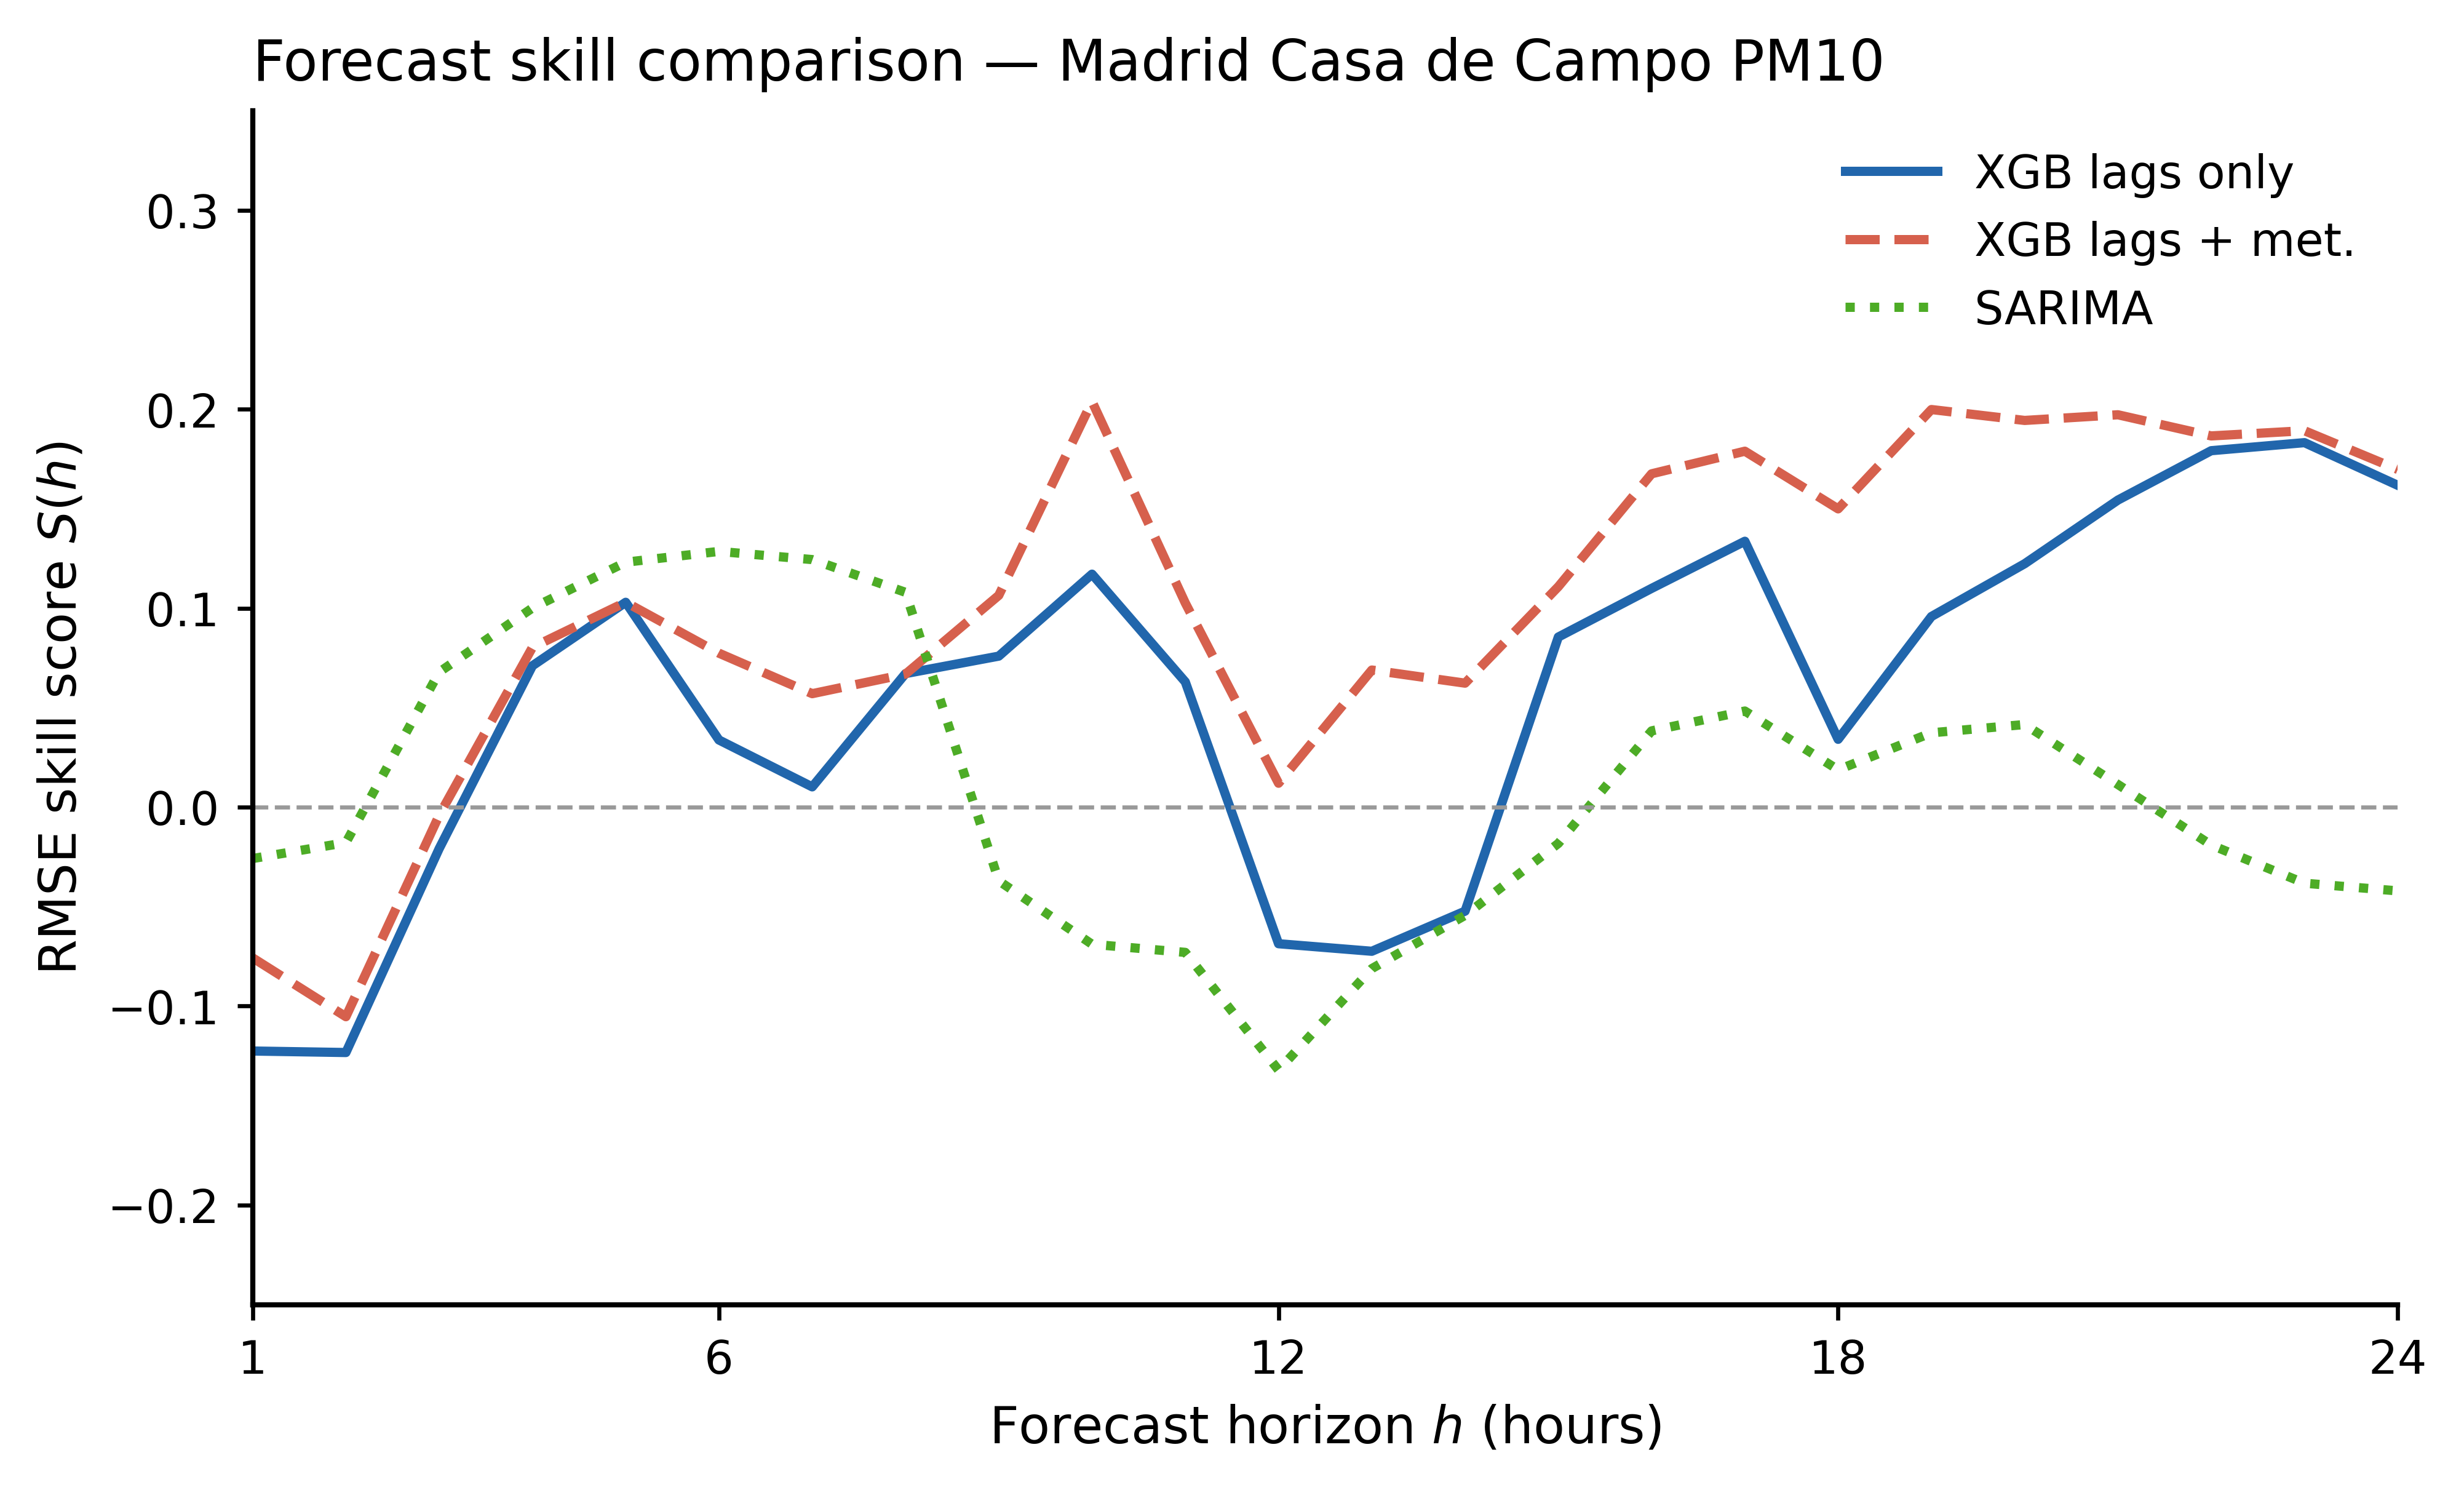
\includegraphics[width=0.85\textwidth]{figures/madrid_figure_skill_curves.png}
  \caption{RMSE skill score $S(h)$ relative to persistence as a function of
    forecast horizon $h$ for Madrid Casa de Campo \PMten{} (2023 evaluation
    window).  Positive values indicate improvement over persistence.
    Blue solid: XGBoost lags only; red dashed: XGBoost lags + met.; green
    dotted: SARIMA.  Horizontal dashed line at $S = 0$.}
  \label{fig:madrid_skill}
\end{figure}

\begin{figure}[htbp]
  \centering
  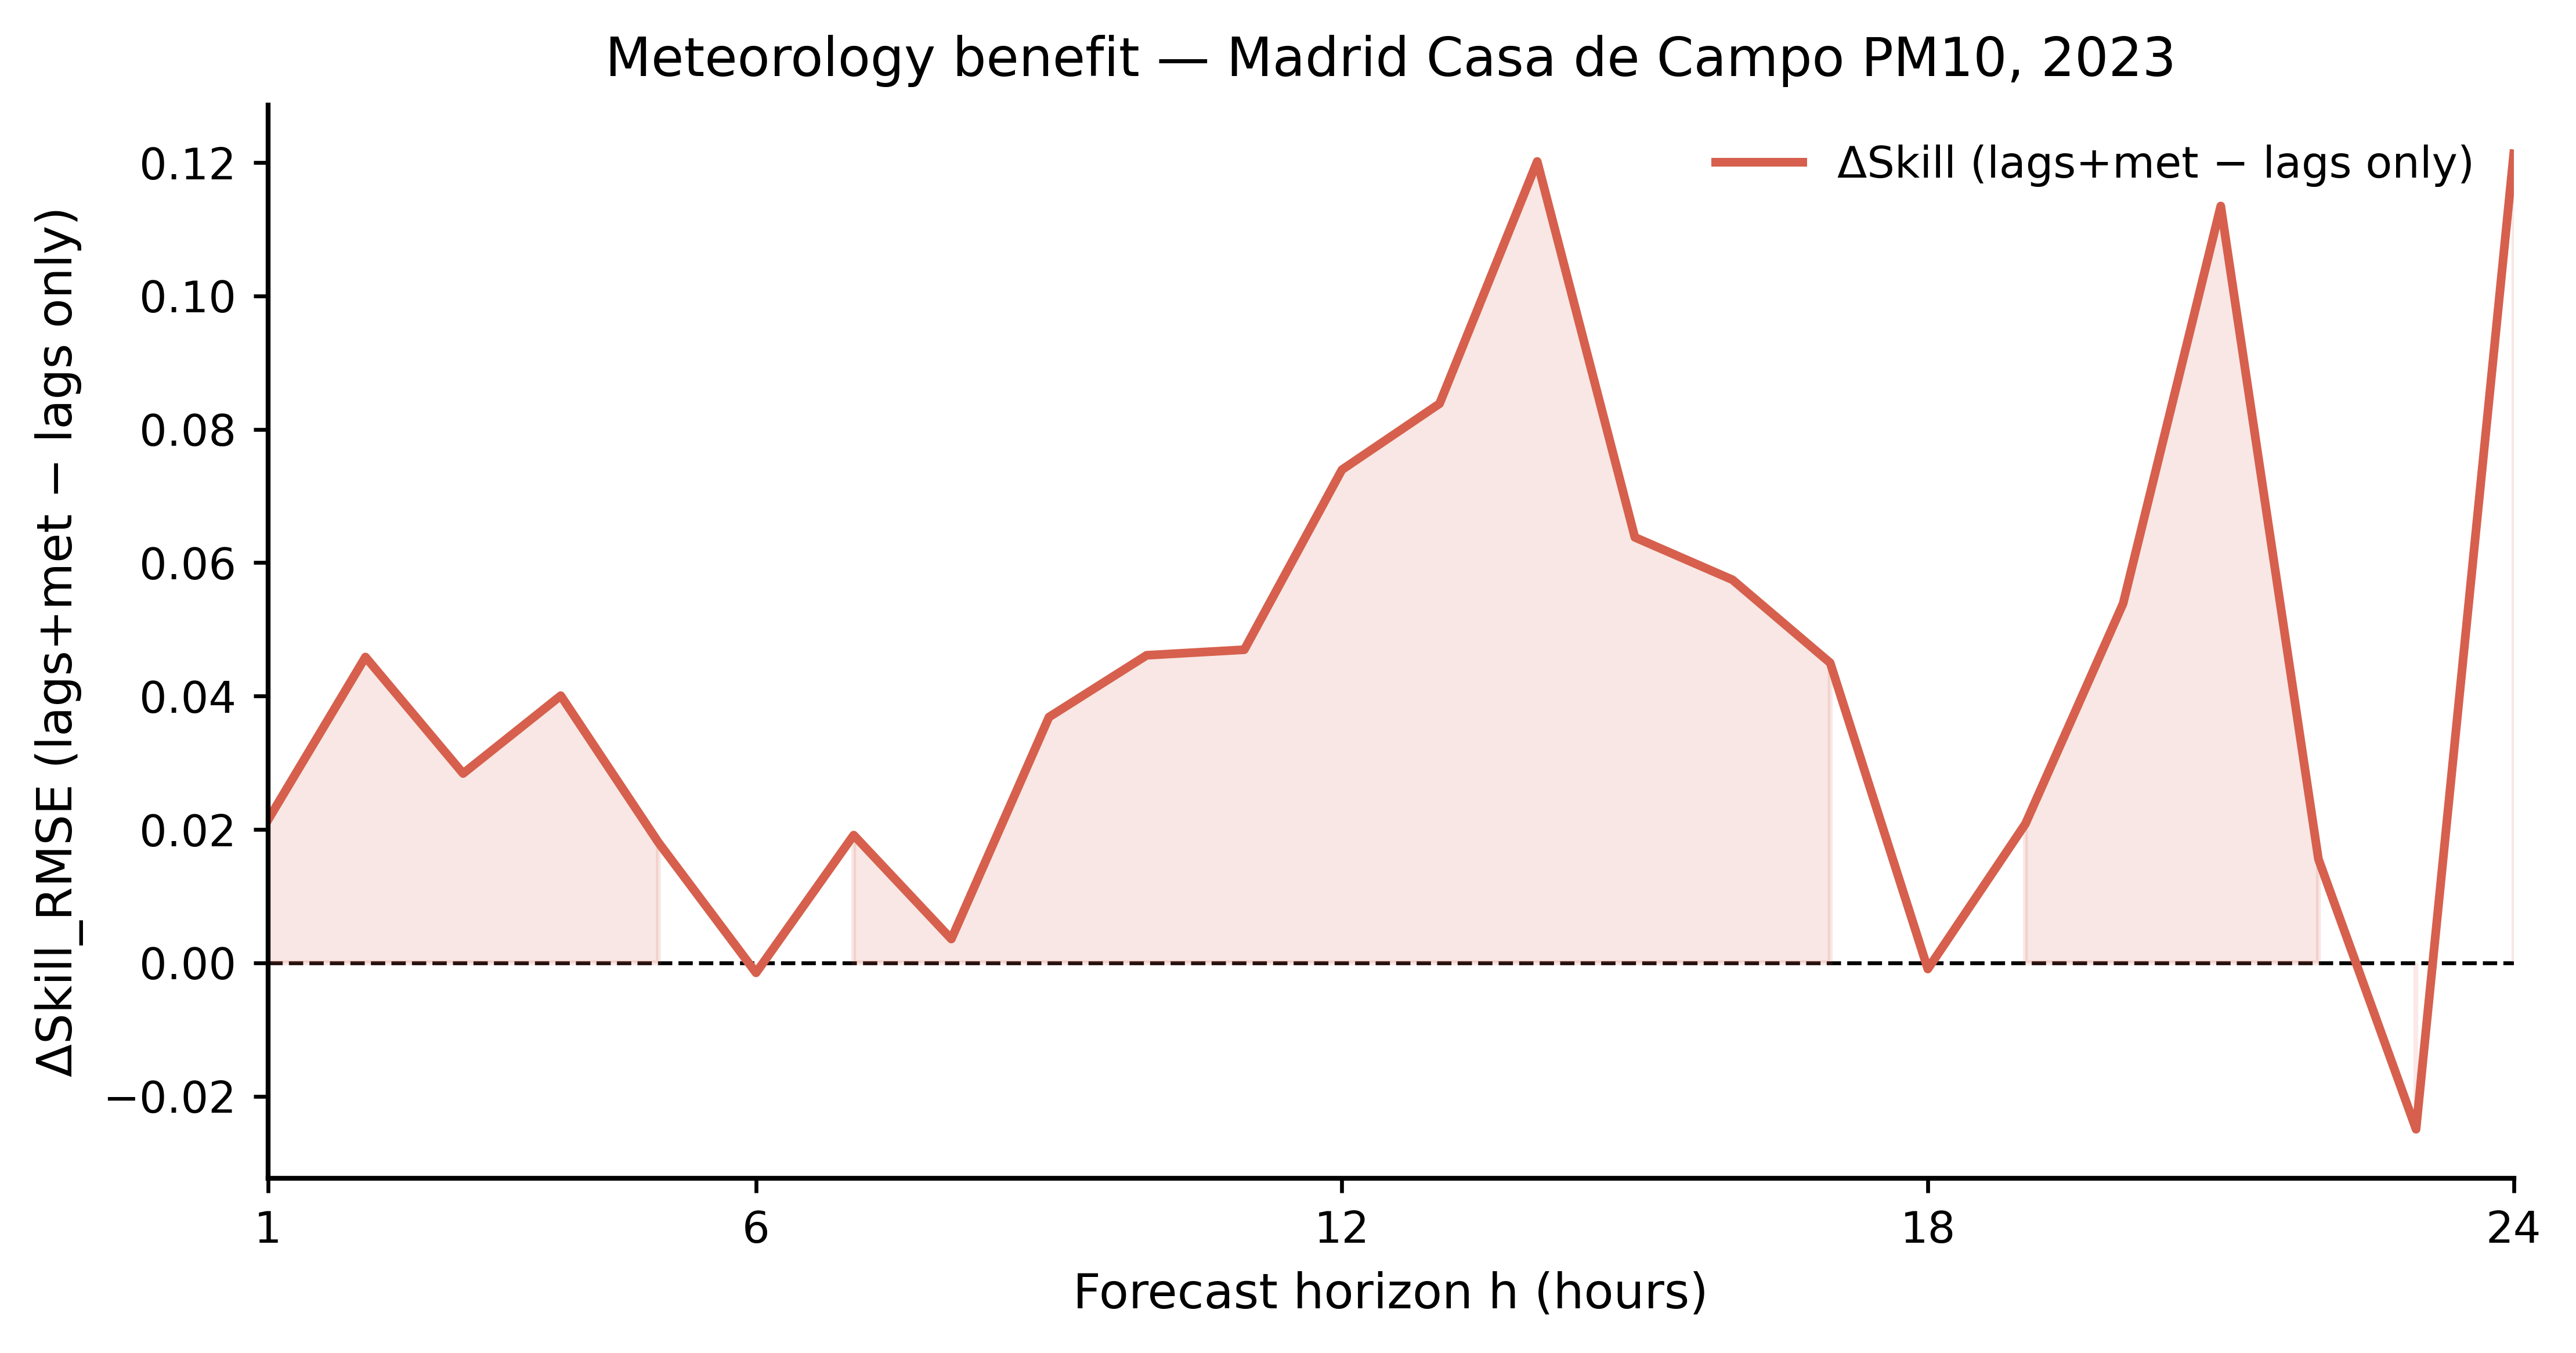
\includegraphics[width=0.85\textwidth]{figures/madrid_figure_delta_skill.png}
  \caption{Pointwise difference in RMSE skill score,
    $\Delta S(h) = S_{\text{lags+met}}(h) - S_{\text{lags only}}(h)$,
    for Madrid Casa de Campo \PMten{}.  Filled areas above zero (shaded red)
    indicate horizons where meteorology improves skill; areas below zero
    (shaded blue) indicate horizons where lags-only is superior.}
  \label{fig:madrid_delta}
\end{figure}

\begin{figure}[htbp]
  \centering
  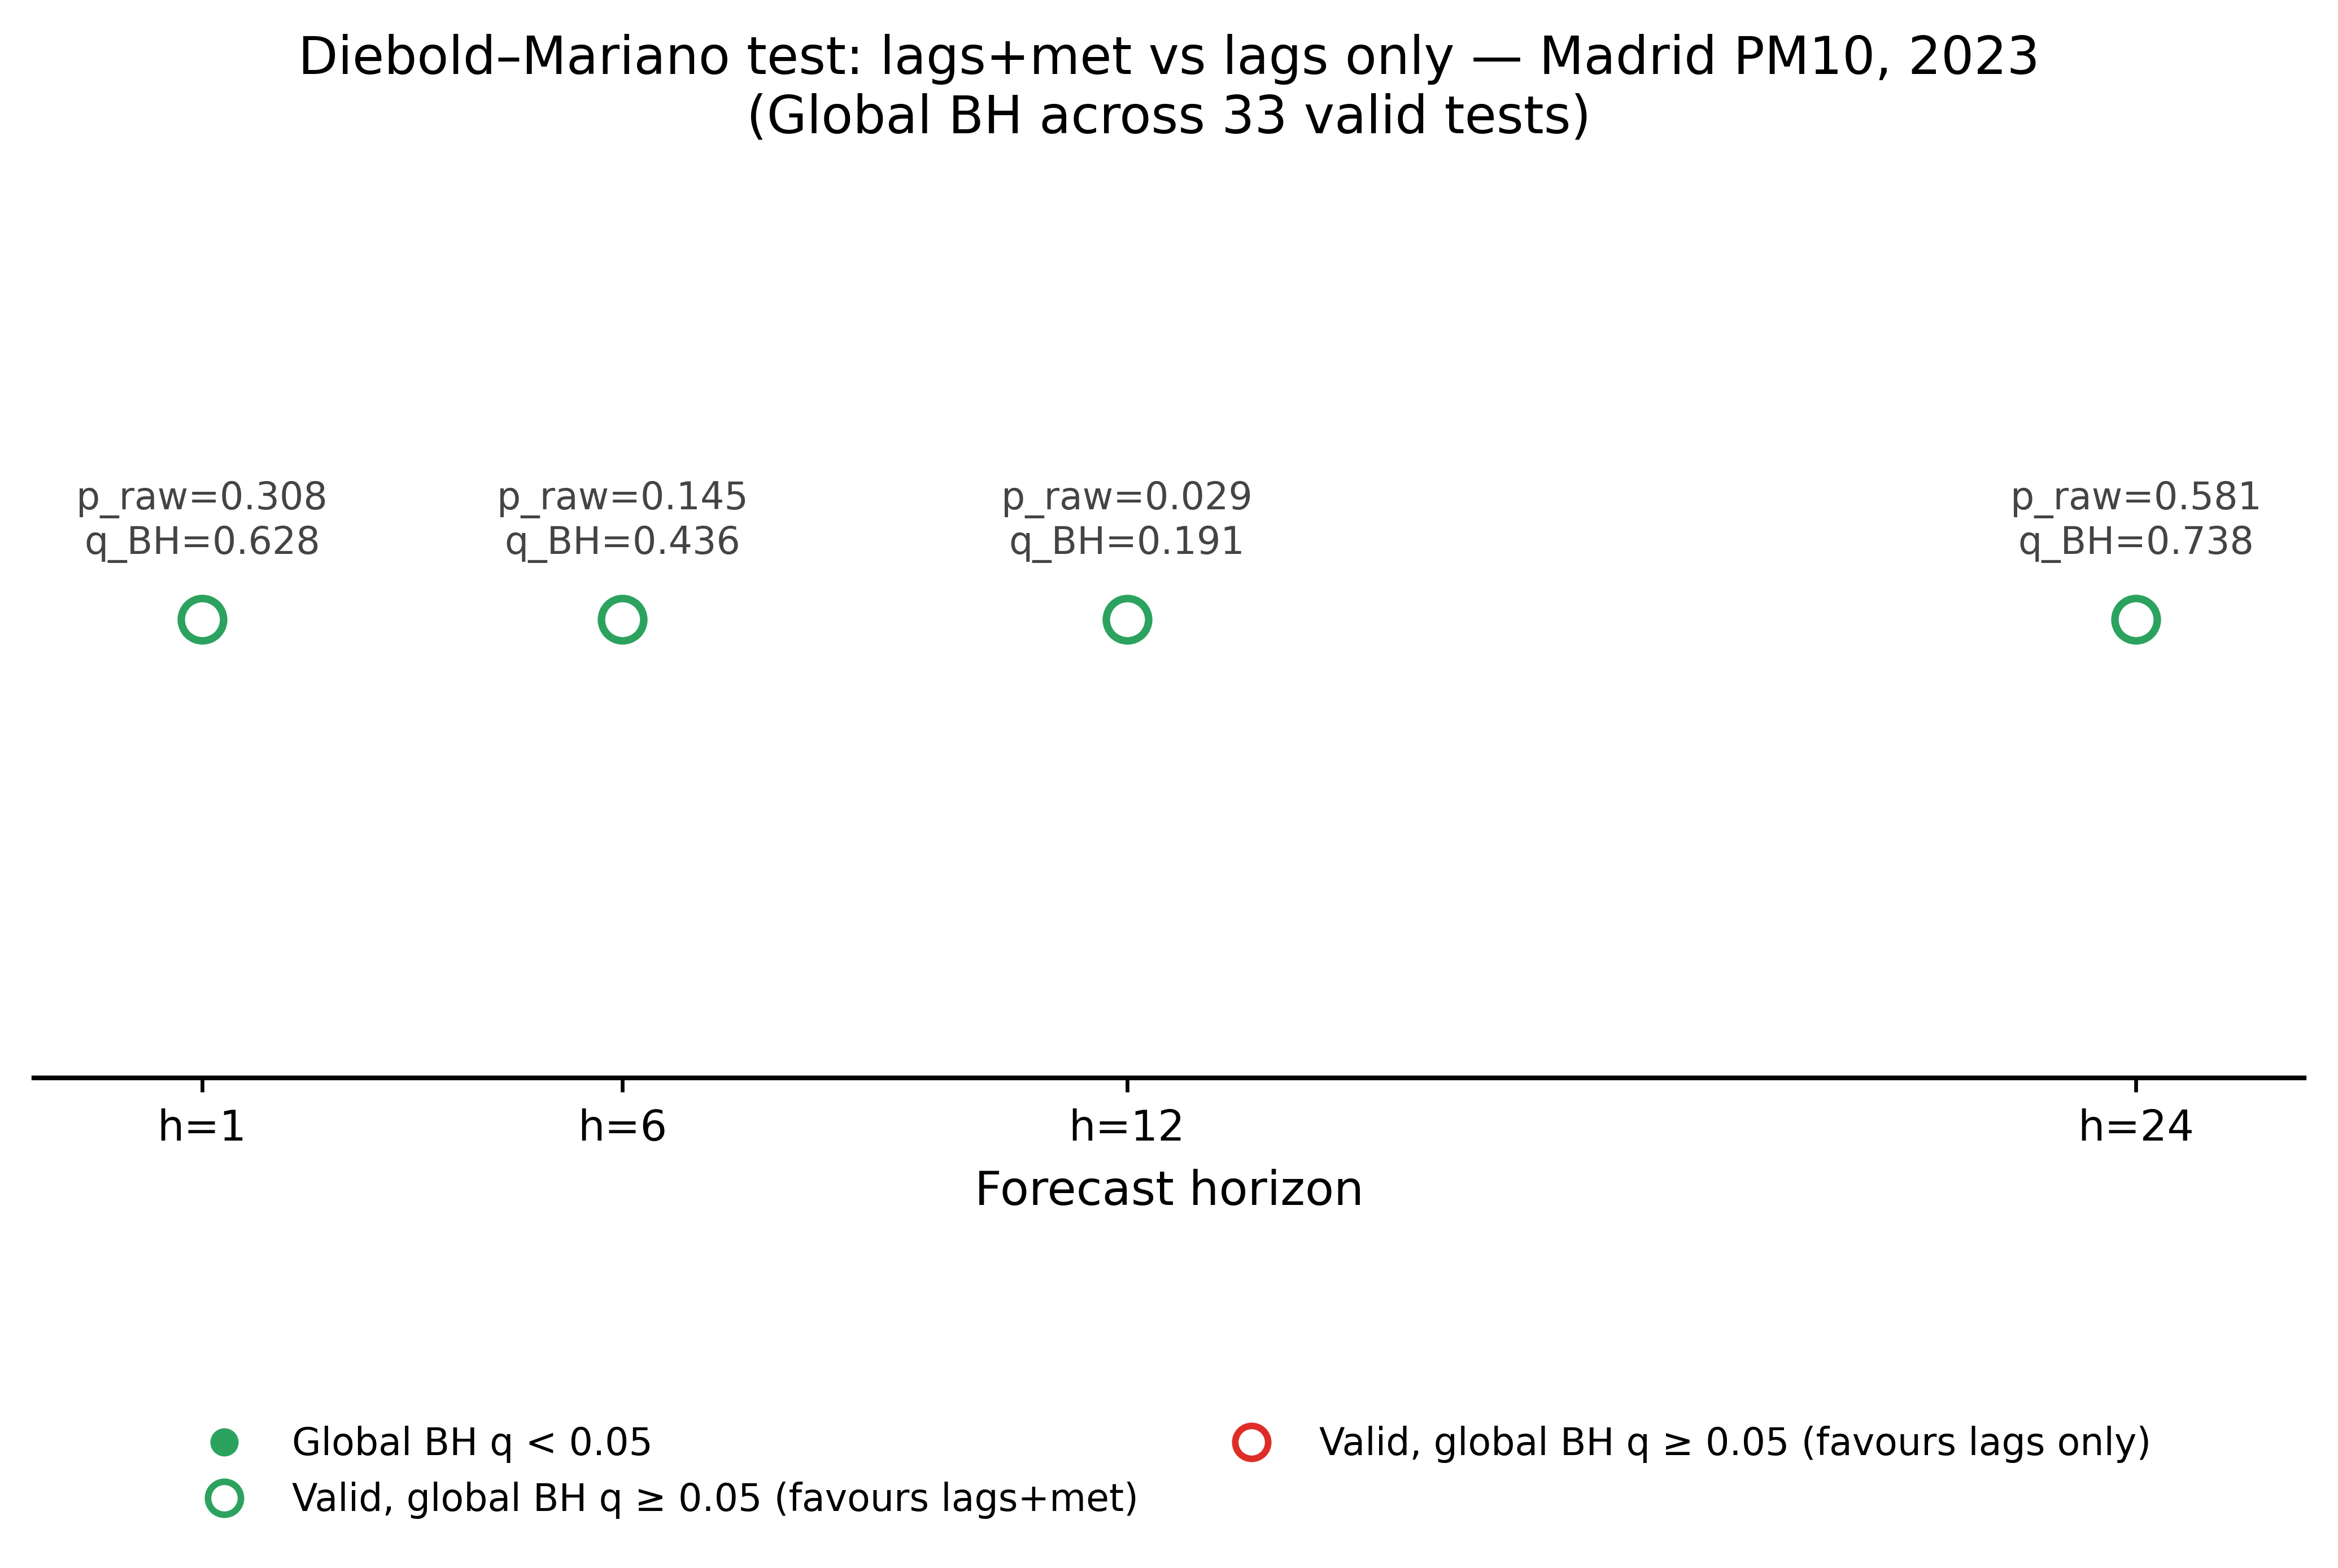
\includegraphics[width=0.75\textwidth]{figures/madrid_figure_dm_significance.png}
  \caption{Diebold--Mariano contrasts for Madrid at $h\in\{1,6,12,24\}$.
    Upward triangles favour lags + met.; downward triangles favour lags only.
    Global multiplicity results are reported in Table~\ref{tab:ireland_dm}; no
    Madrid comparison is globally BH-significant.}
  \label{fig:madrid_dm}
\end{figure}

\begin{figure}[htbp]
  \centering
  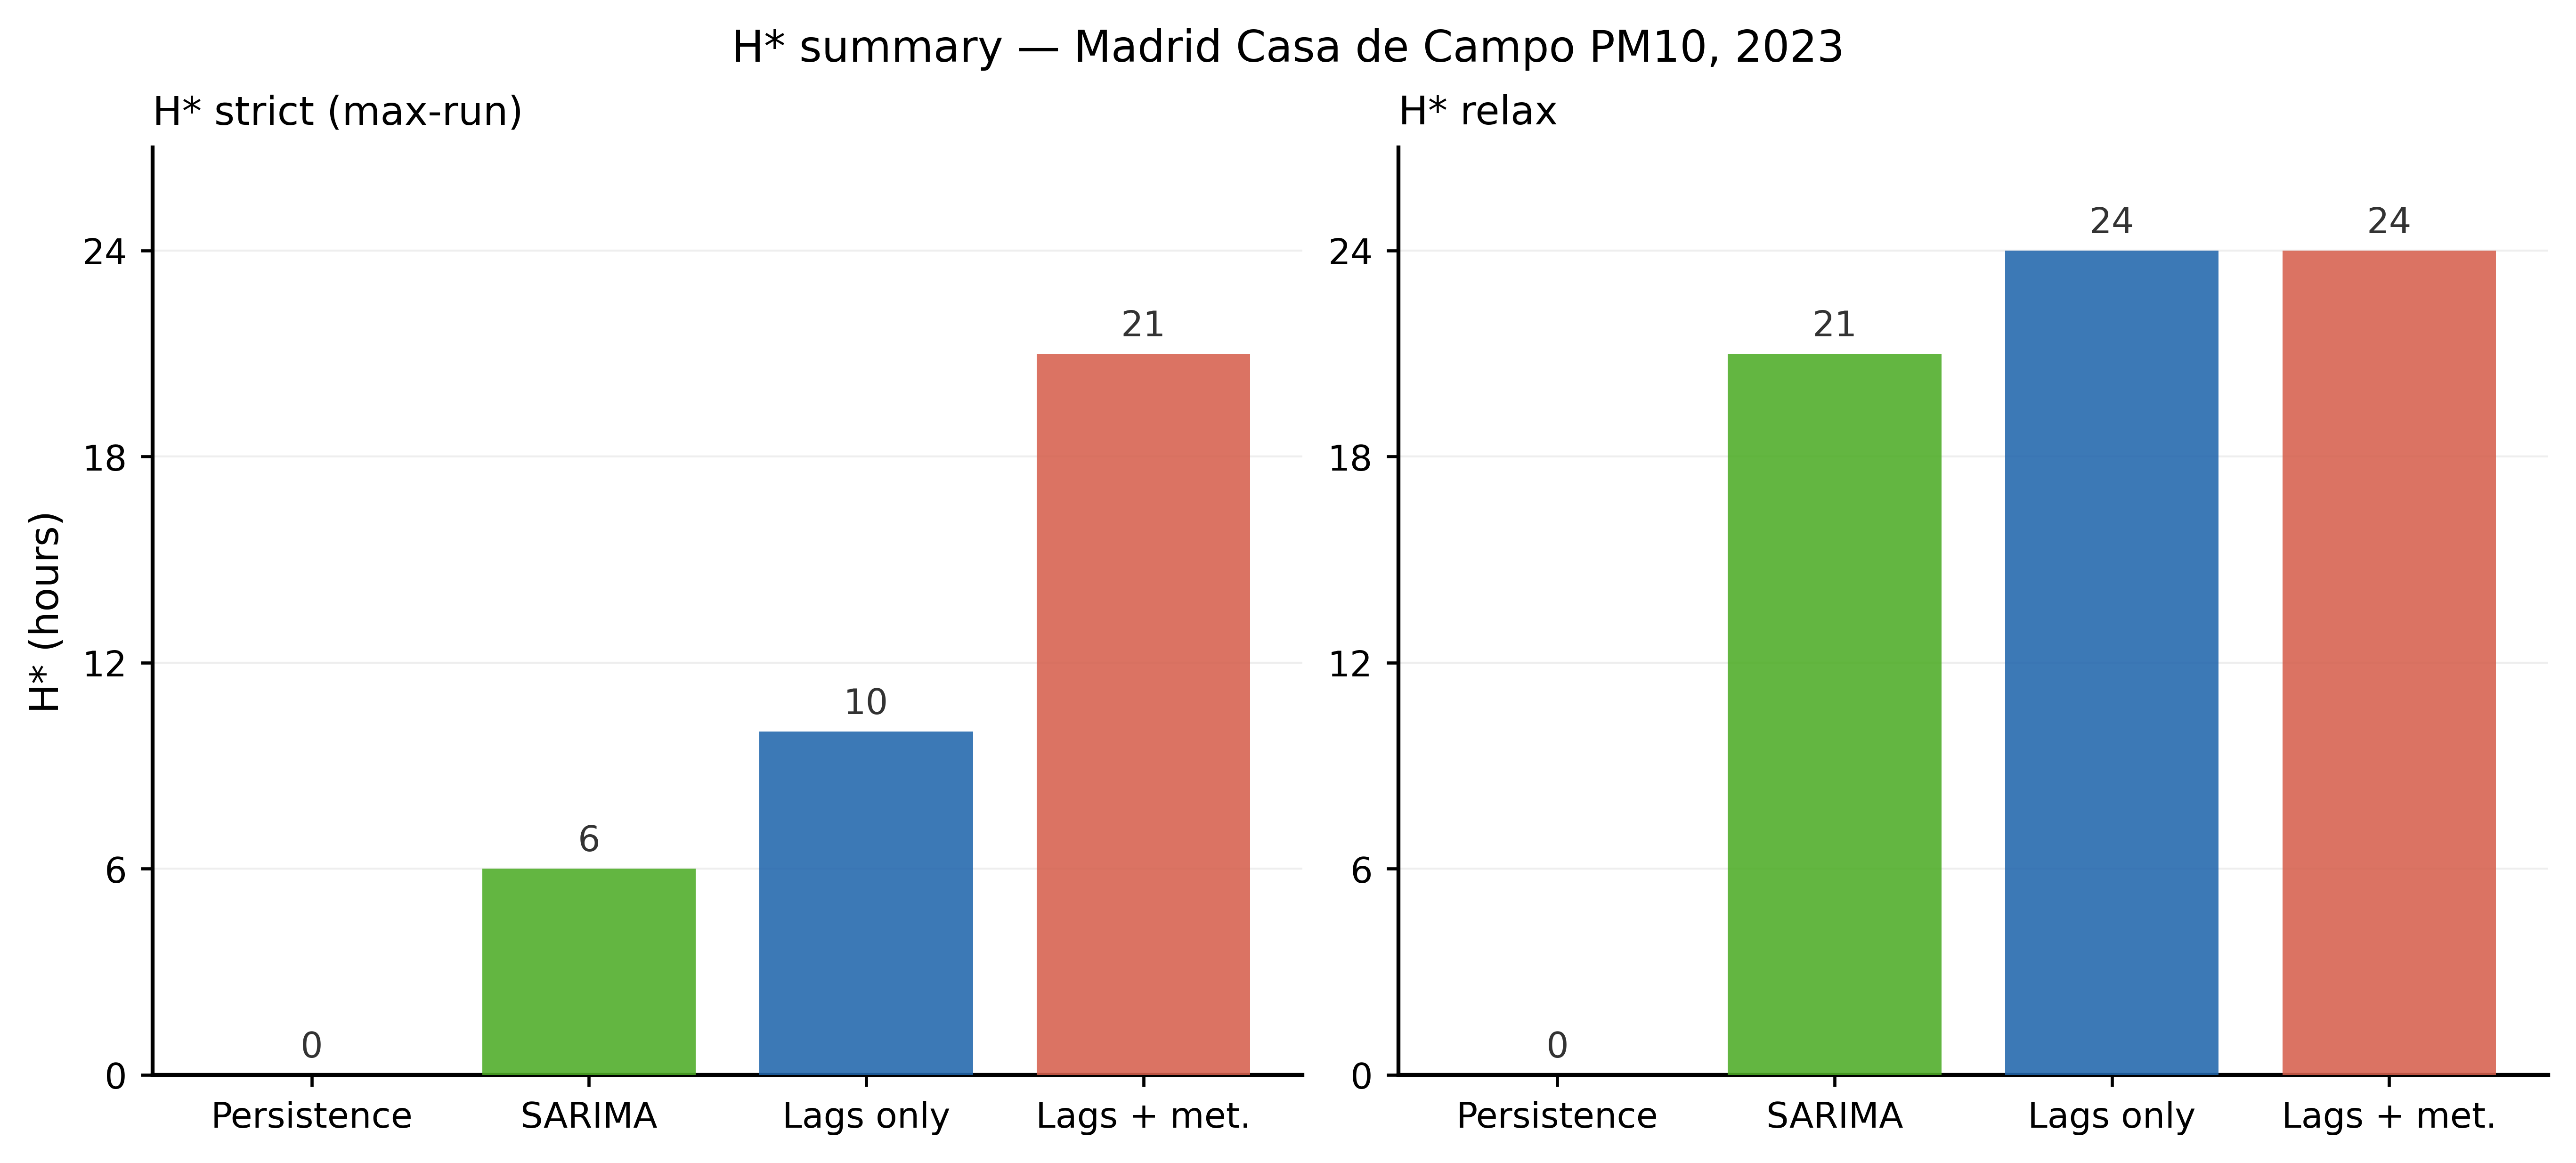
\includegraphics[width=0.88\textwidth]{figures/madrid_figure_hstar_summary.png}
  \caption{$H^*$ summary bar chart for Madrid Casa de Campo.  Left panel:
    $H^*_{\text{strict}}$; right panel: $H^*_{\text{relax}}$.  Grey:
    persistence; green: SARIMA; blue: XGBoost lags only; red: XGBoost lags +
    met.  Numbers above each bar show the value in hours.}
  \label{fig:madrid_hstar}
\end{figure}

% ── Ireland figures ───────────────────────────────────────────────────────────

\begin{figure}[htbp]
  \centering
  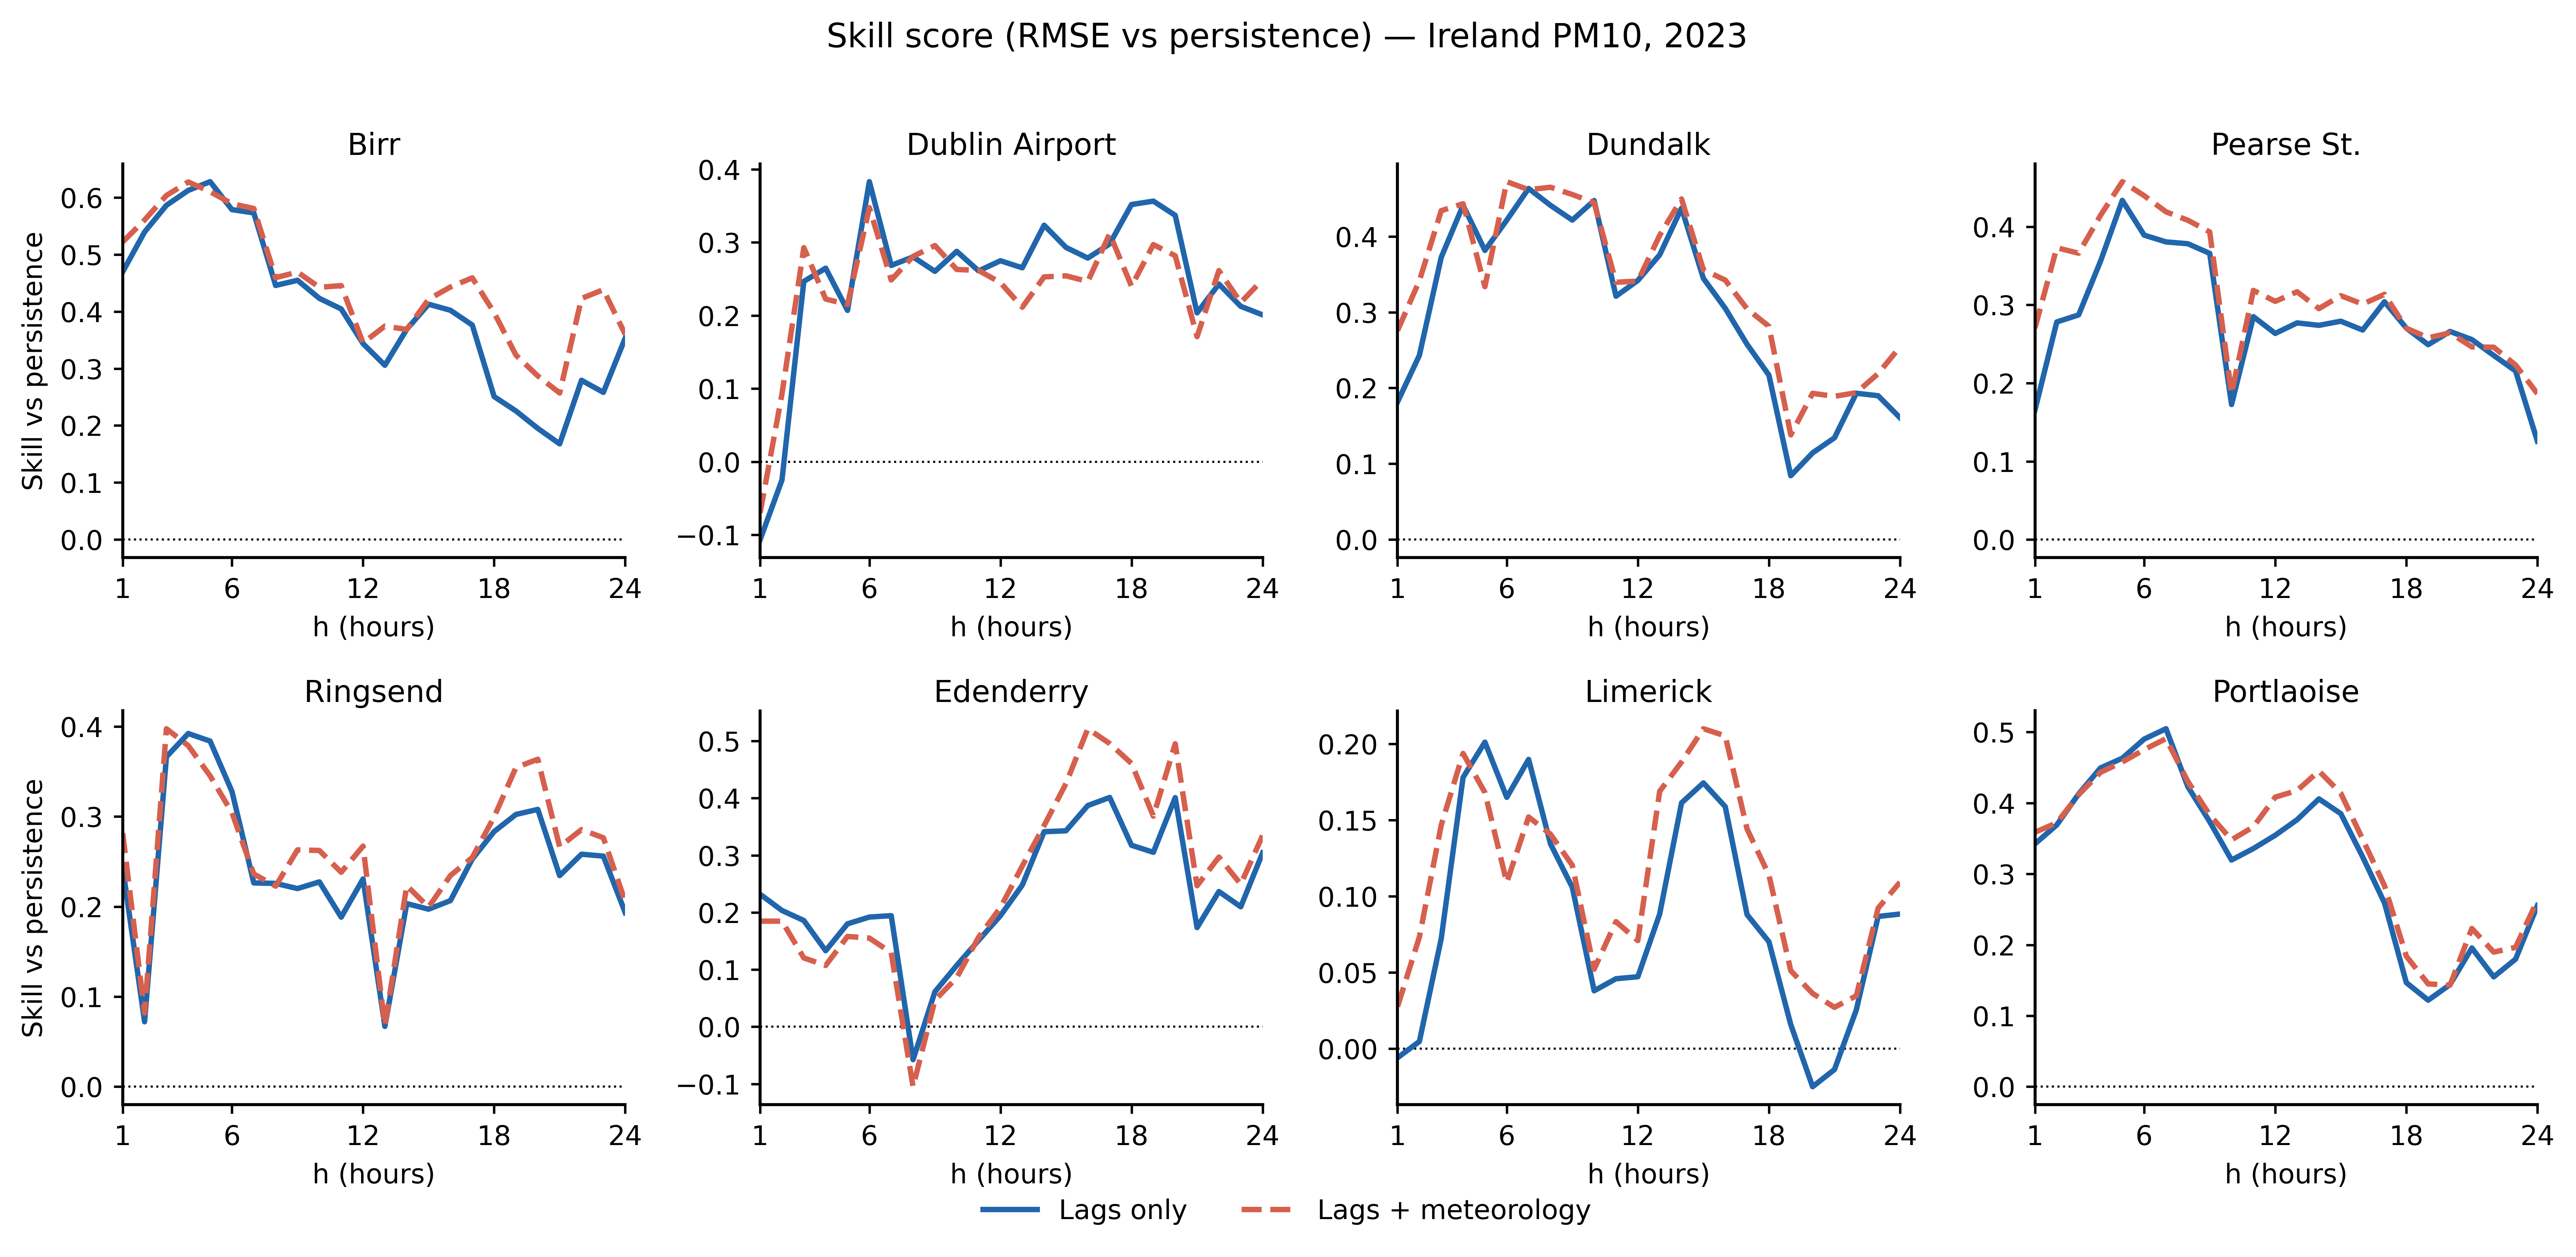
\includegraphics[width=\textwidth]{figures/ireland_figure_skill_by_station.png}
  \caption{RMSE skill score $S(h)$ relative to persistence as a function of
    forecast horizon $h$ for all eight Irish \PMten{} monitoring stations
    (2023 evaluation window).  Each panel shows one station.  Blue solid:
    XGBoost lags only; red dashed: XGBoost lags + meteorology.  Horizontal
    dotted line at $S = 0$.}
  \label{fig:ireland_skill}
\end{figure}

\begin{figure}[htbp]
  \centering
  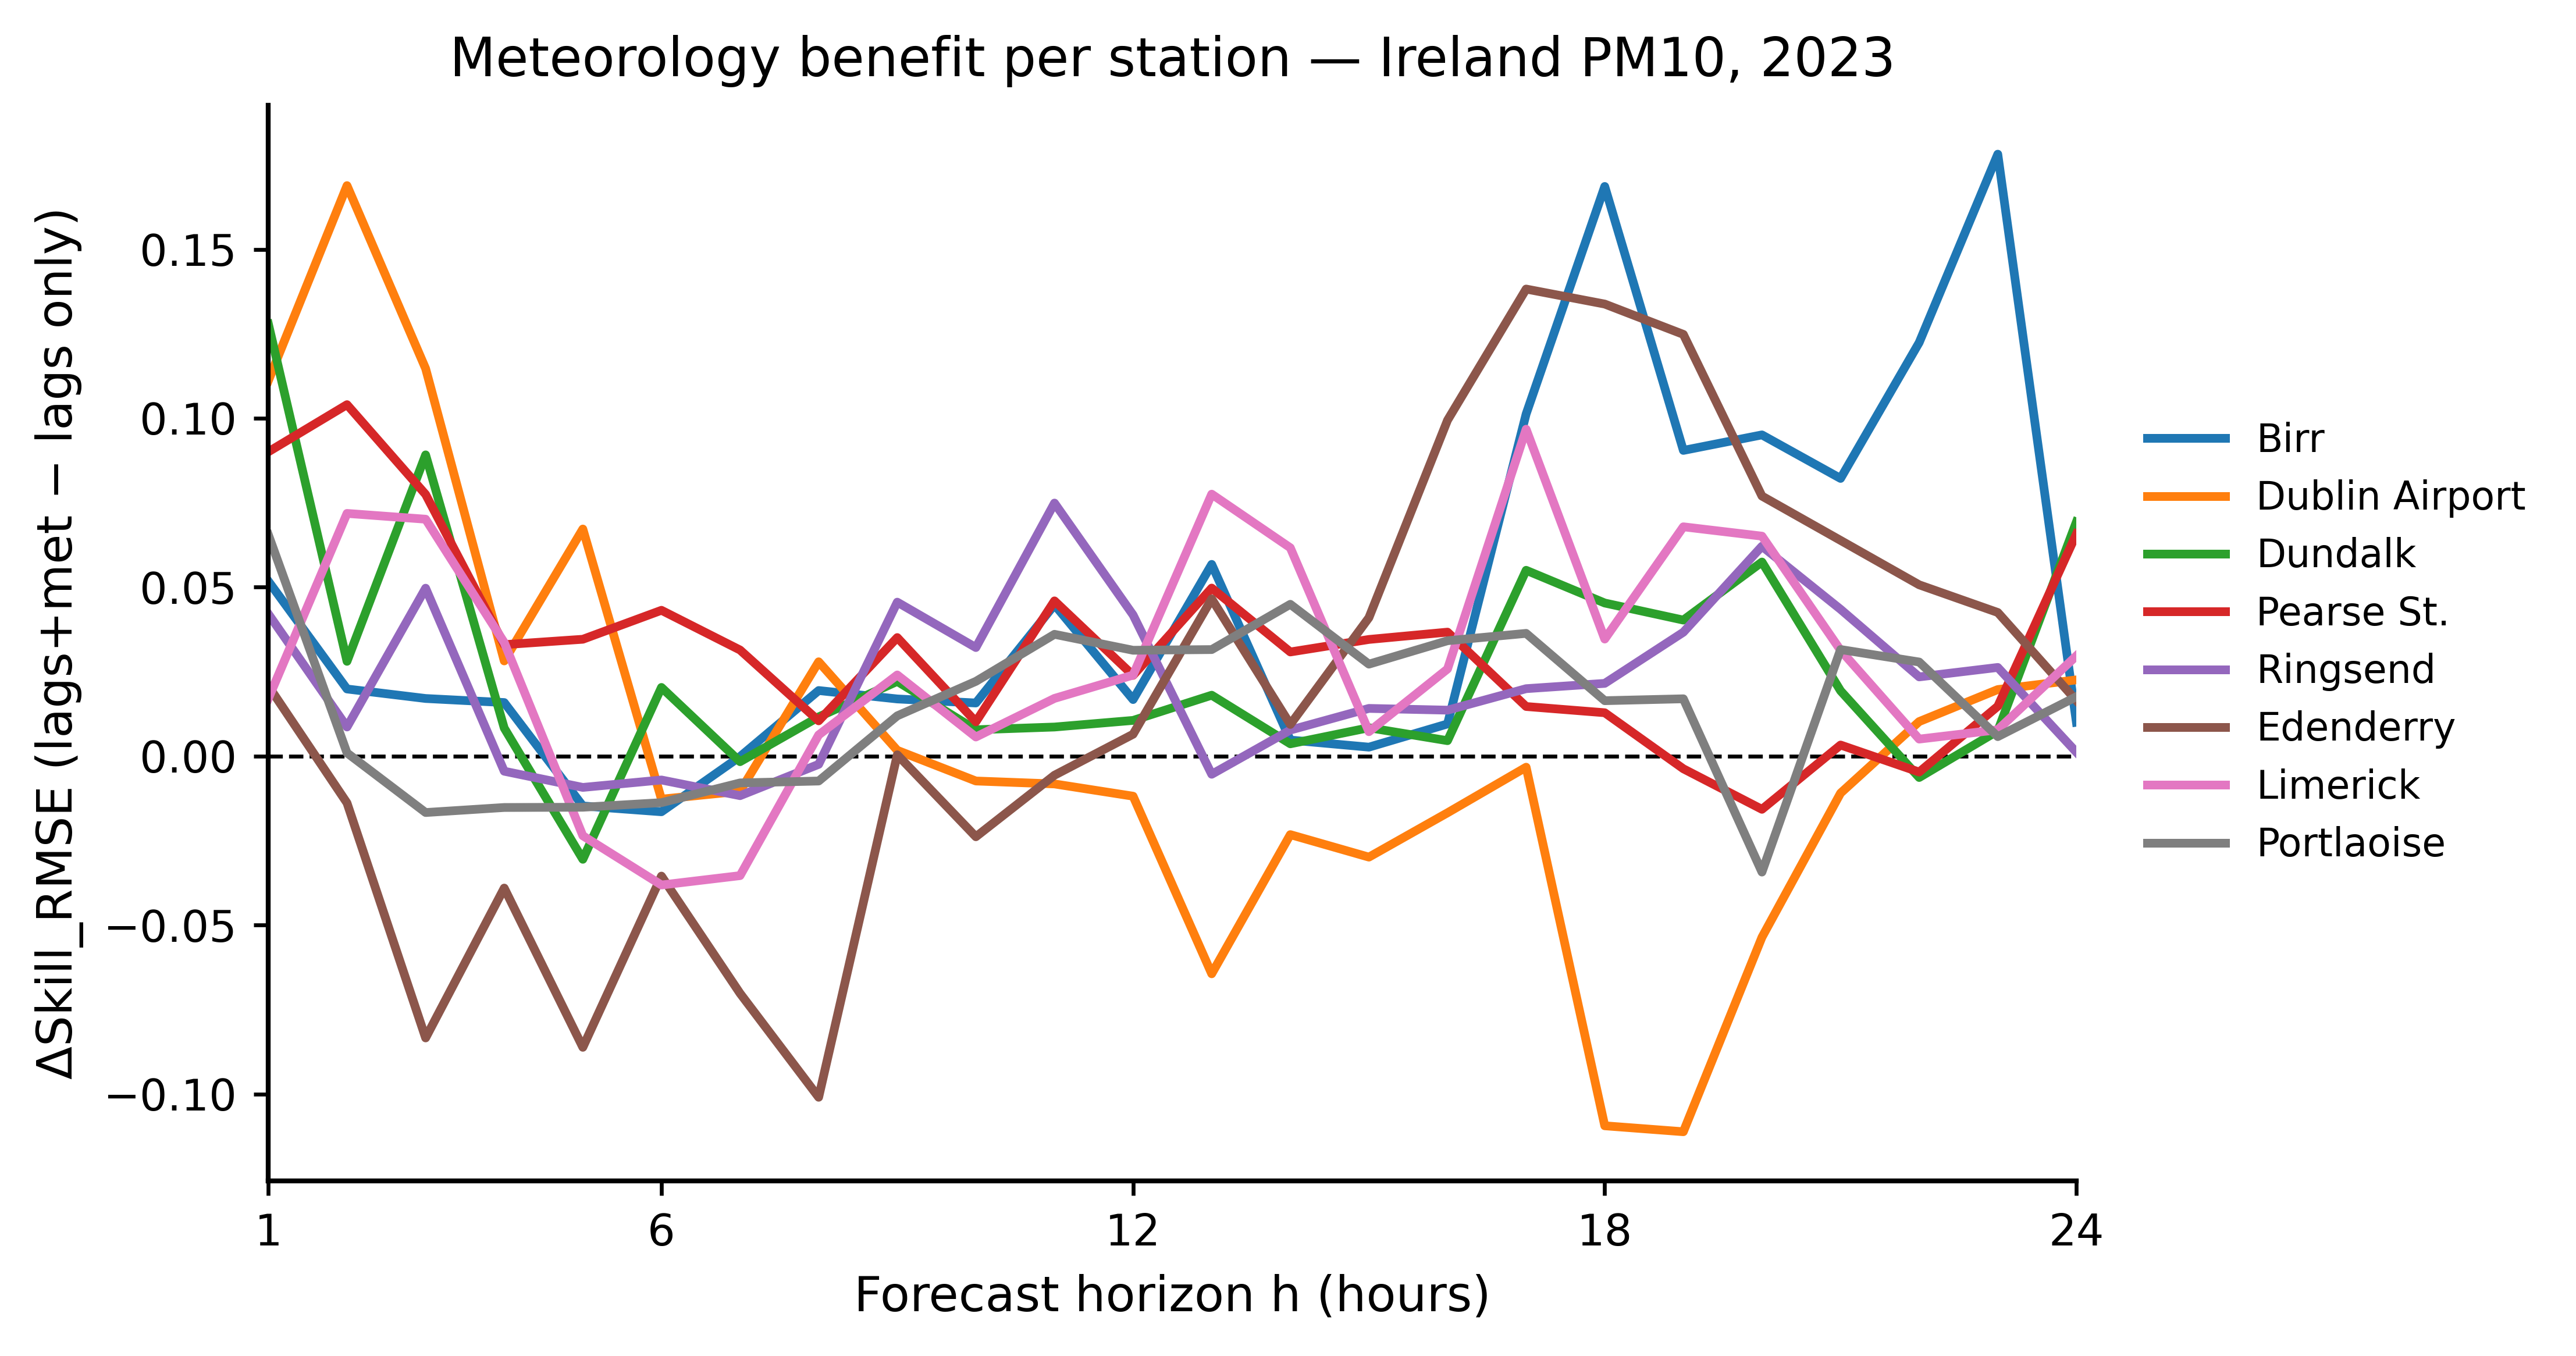
\includegraphics[width=0.85\textwidth]{figures/ireland_figure_delta_skill.png}
  \caption{Pointwise meteorology benefit $\Delta S(h) = S_{\text{lags+met}}(h)
    - S_{\text{lags only}}(h)$ for each Irish station (one coloured line per
    station).  The horizontal dashed line marks $\Delta S = 0$.  Values near
    zero at most stations and most horizons indicate that lags-only XGBoost
    already captures the dominant predictable variance.}
  \label{fig:ireland_delta}
\end{figure}

\begin{figure}[htbp]
  \centering
  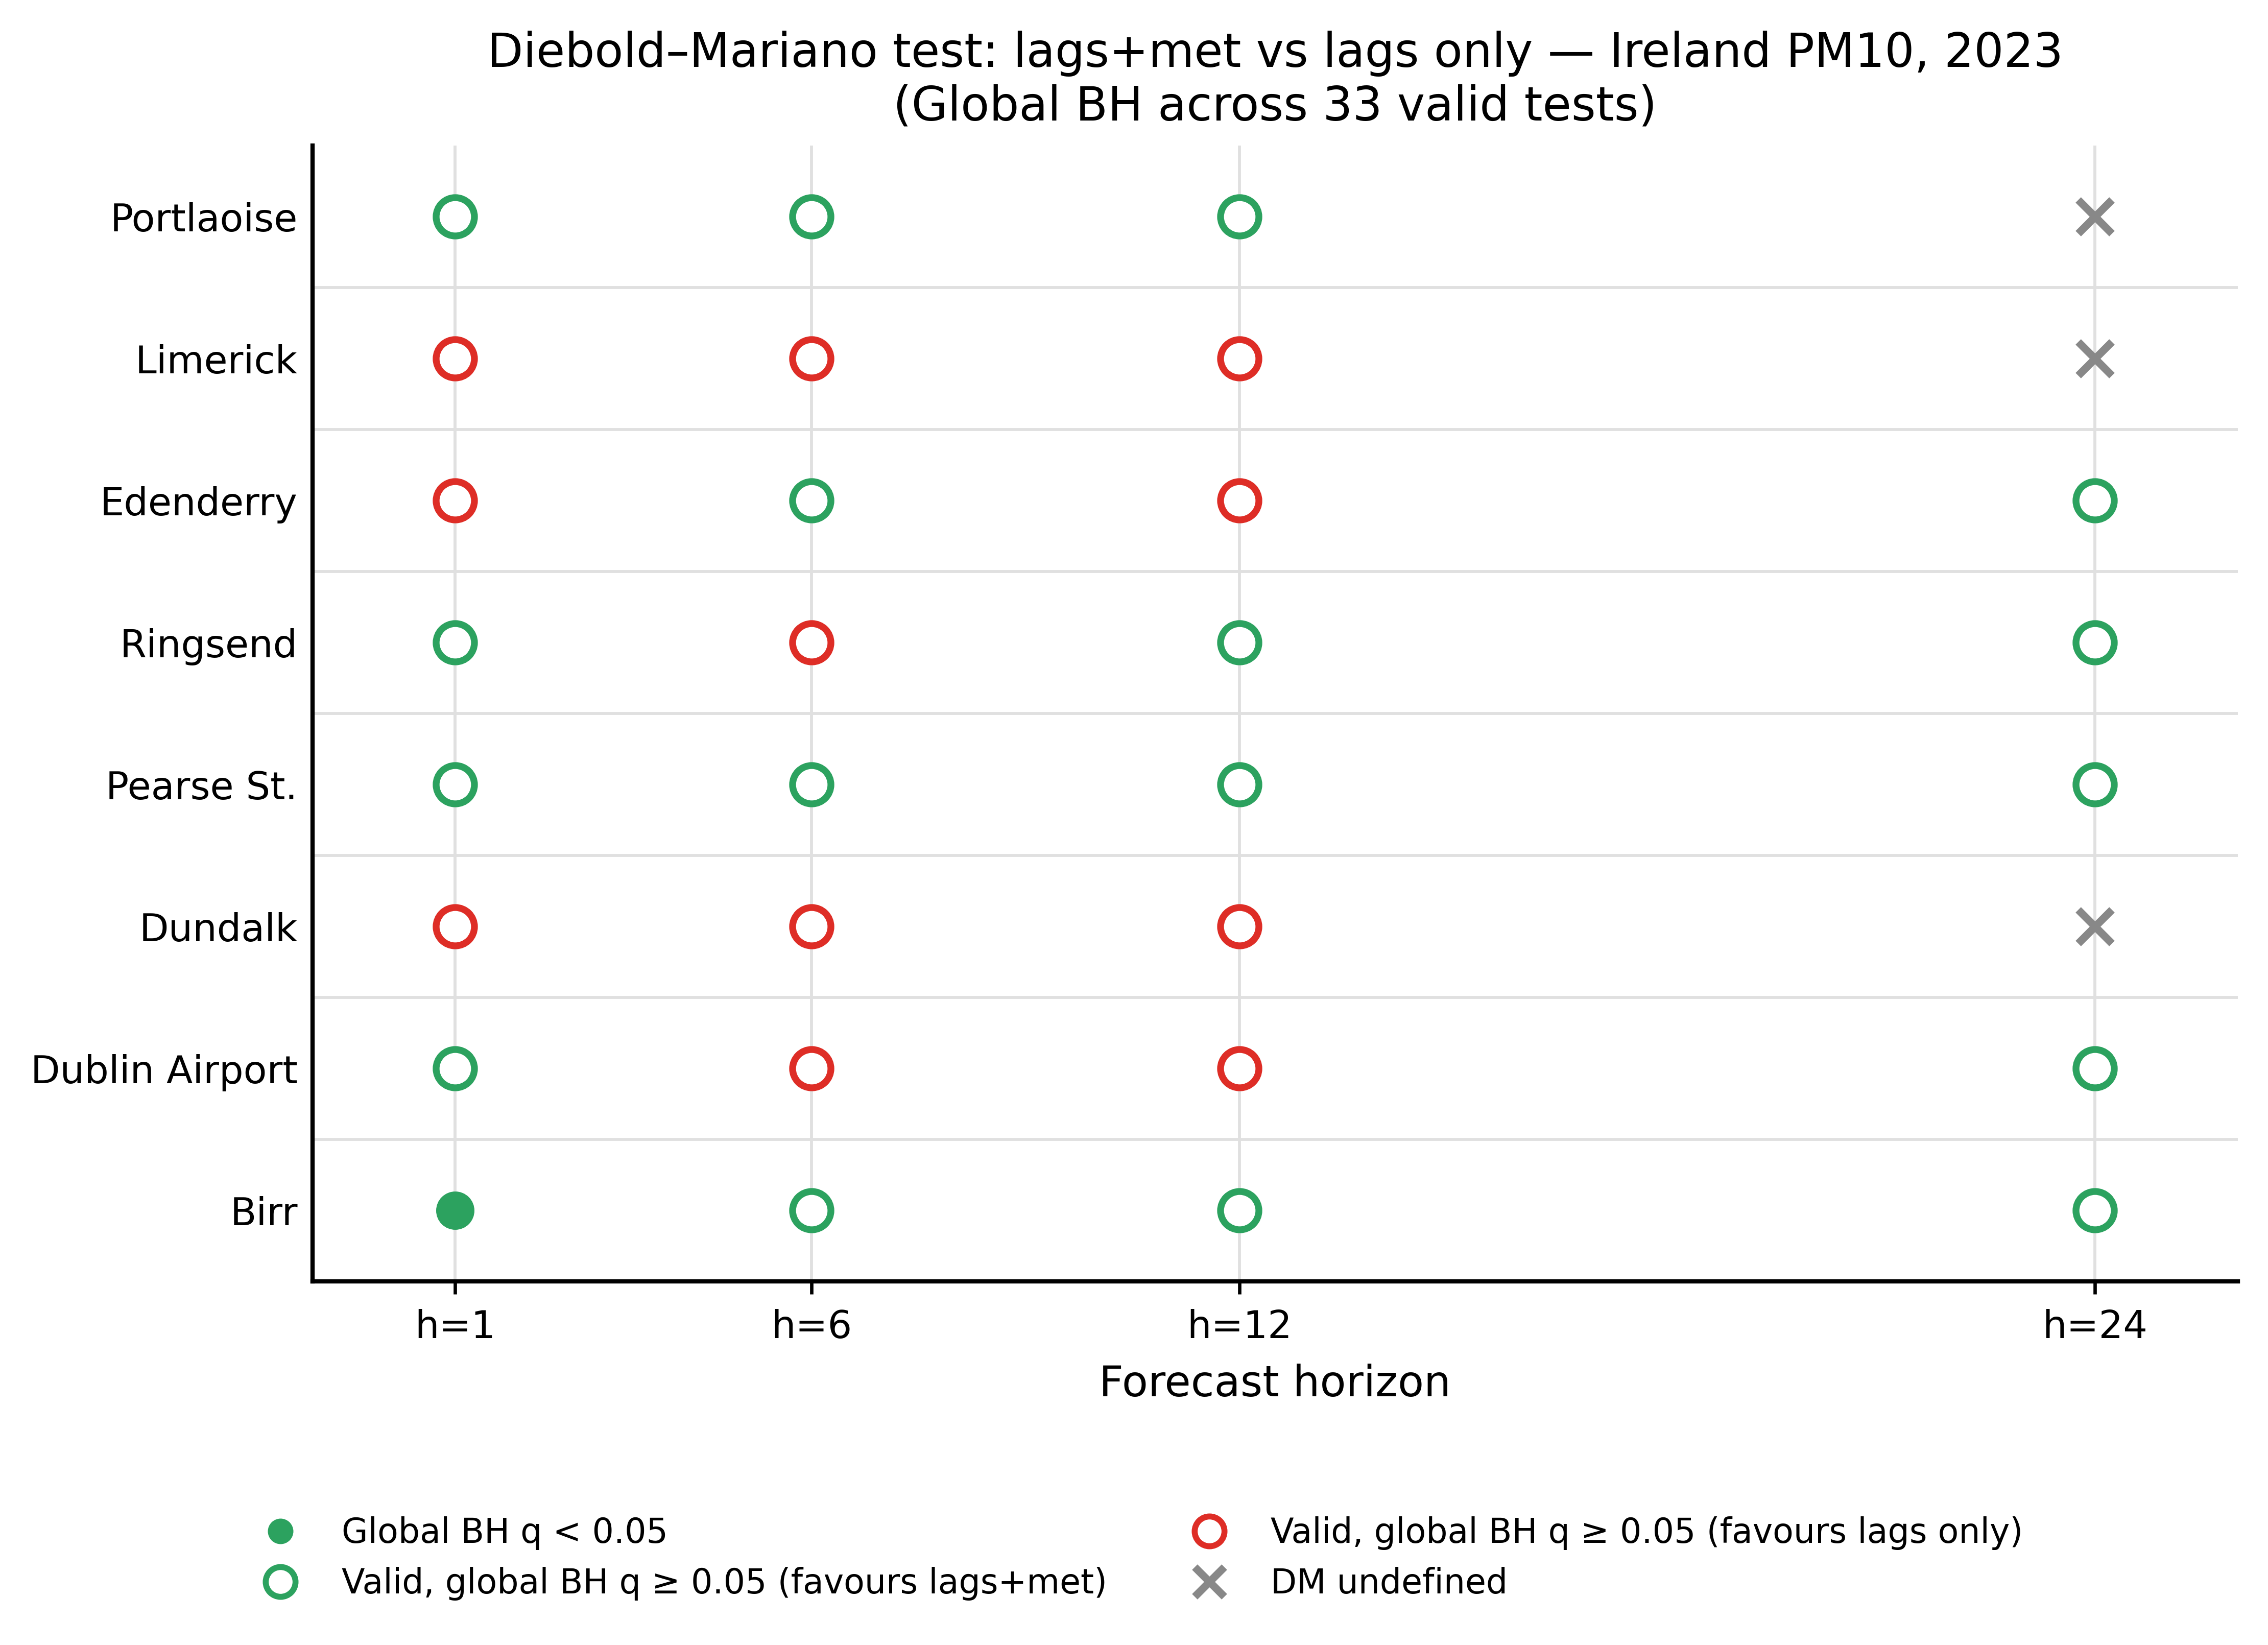
\includegraphics[width=0.78\textwidth]{figures/ireland_figure_dm_significance.png}
  \caption{Diebold--Mariano contrasts for Ireland: lags + met.\ vs.\ lags only
    at $h\in\{1,6,12,24\}$.  Each row is a station and each column a horizon.
    Upward triangles favour lags + met.; downward triangles favour lags only.
    Global multiplicity and invalid-test handling are reported in
    Table~\ref{tab:ireland_dm}; after global BH over the 33 valid tests, only
    Birr $h=1$ remains significant.}
  \label{fig:ireland_dm}
\end{figure}

\begin{figure}[htbp]
  \centering
  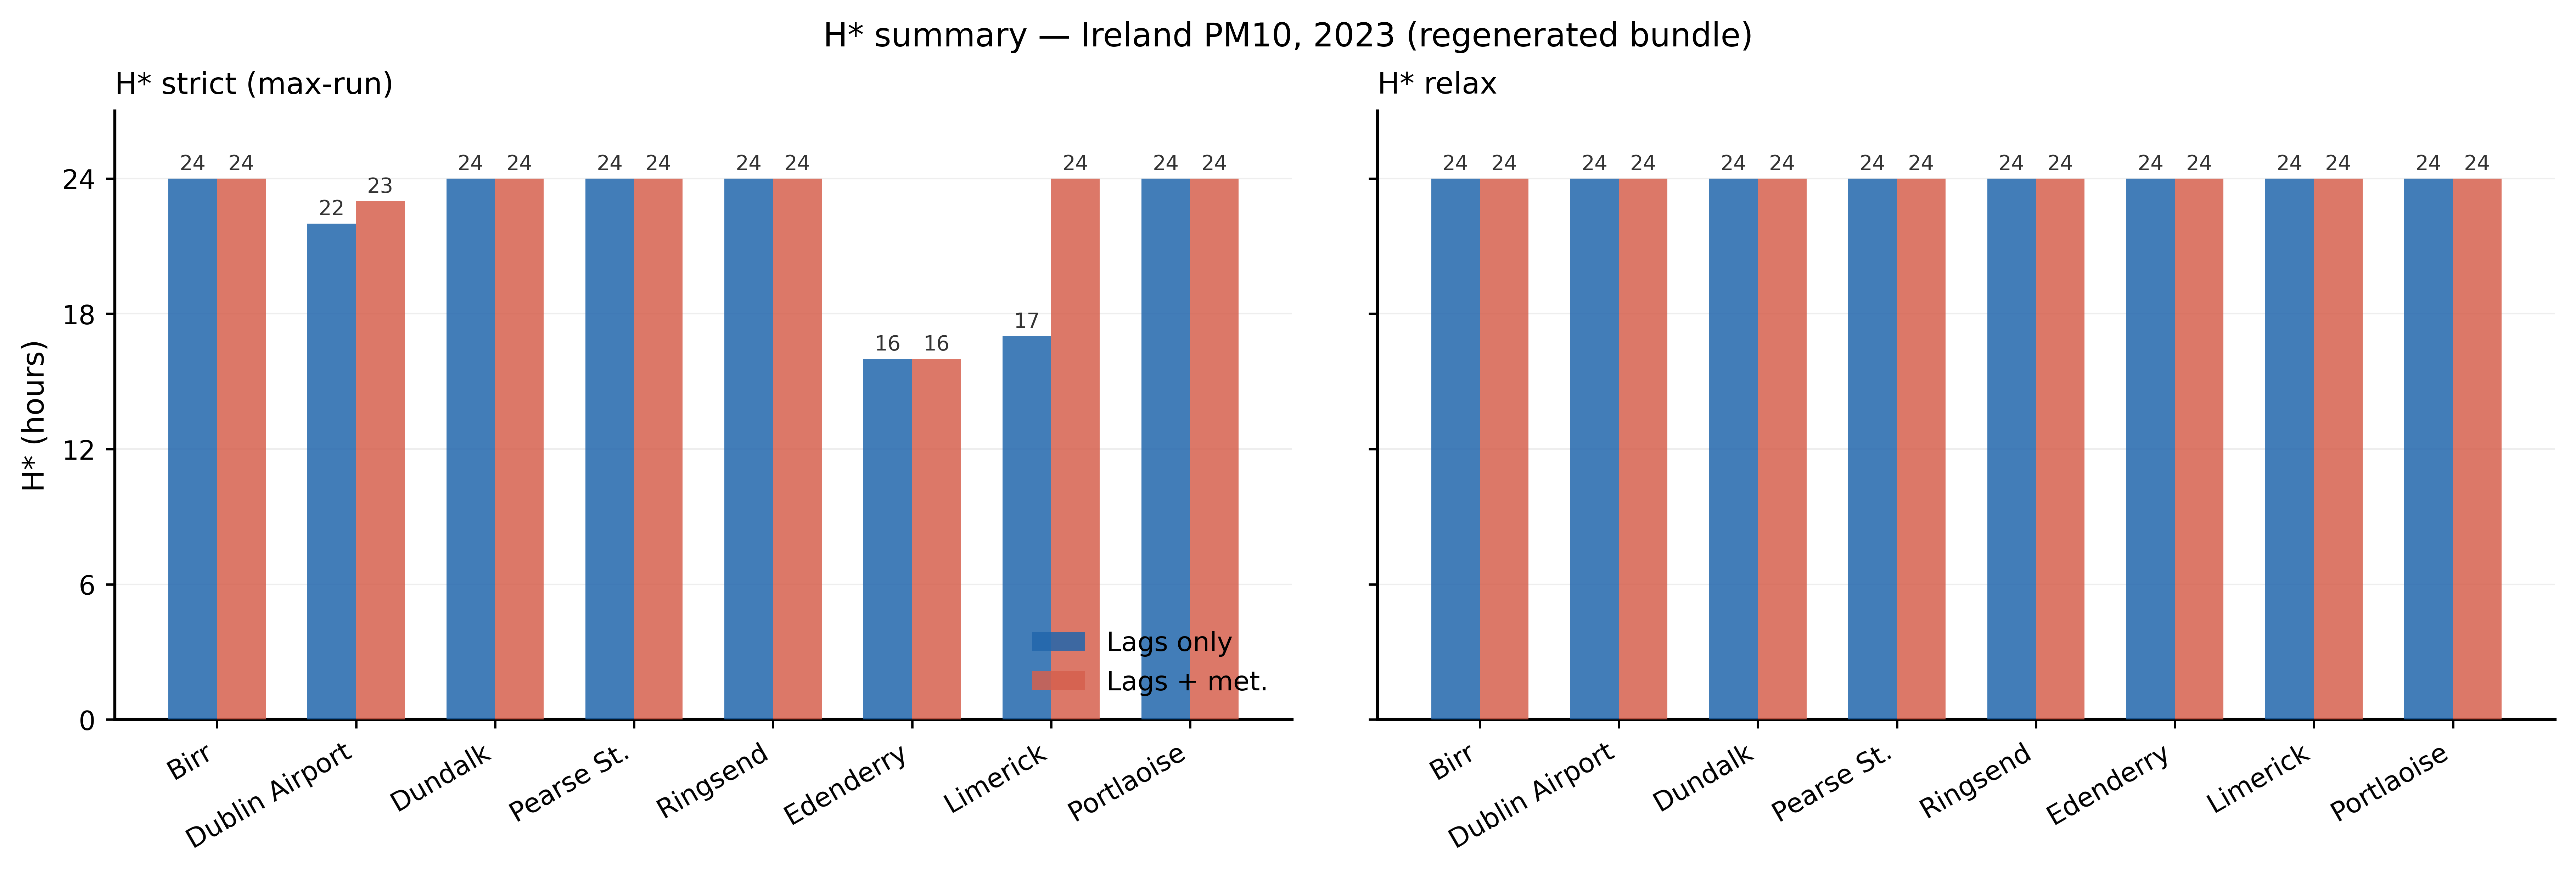
\includegraphics[width=\textwidth]{figures/ireland_figure_hstar_summary.png}
  \caption{$H^*$ summary for all eight Irish stations.  Left panel:
    $H^*_{\text{strict}}$; right panel: $H^*_{\text{relax}}$.  Blue bars:
    XGBoost lags only; red bars: XGBoost lags + meteorology.  Numbers above
    each bar show the value in hours.}
  \label{fig:ireland_hstar}
\end{figure}

% ── ρ₁ vs ΔH* scatter ────────────────────────────────────────────────────────
% (Omitted from the main manuscript in the timestamp-safe canonicalized revision.)

% ─────────────────────────────────────────────────────────────────────────────
% Bibliography
% ─────────────────────────────────────────────────────────────────────────────

\newpage
\bibliography{references}

\end{document}
